\documentclass{article}

\usepackage{iclr2025_conference}

\usepackage[utf8]{inputenc}
\usepackage[T1]{fontenc}
\usepackage{hyperref}
\usepackage{url}
\usepackage{booktabs}
\usepackage{amsfonts}
\usepackage{amsmath}
\usepackage{amssymb}
\usepackage{nicefrac}
\usepackage{microtype}
\usepackage{xcolor}
\usepackage{graphicx}
\usepackage{array}
\usepackage{flafter}

\input{math_commands.tex}

\title{Endpoint Ranking Does Not Imply Planning: Auditing Cost Geometry in LeWM}

\newcommand{\zgoal}{z_g}
\newcommand{\zhatH}{\hat{z}_H}
\newcommand{\Cmodel}{C_\text{model}}
\newcommand{\Rendpoint}{R_\text{endpoint}}
\newcommand{\Rpool}{R_\text{pool}}
\newcommand{\DeltaCEM}{\Delta_\text{CEM}}
\newcolumntype{L}[1]{>{\raggedright\arraybackslash}p{#1}}

% REVISION: addresses W1 -- abstract and introduction scope narrowed.
% REVISION: addresses W2 -- mechanism-attribution subsection added in Section 4.
% REVISION: addresses W3 -- Cube full projected-CEM table updated with 50-pair, three-seed Phase E results.
% REVISION: addresses W4 -- MPPI cross-optimizer discussion added in Section 8.
% REVISION: addresses W5 -- privilege-free monitoring discussion added in Section 8.
% REVISION: addresses W1/W3/W4 -- limitations updated in Section 9.

\begin{document}

\begin{abstract}
LeWM-style latent planners that optimize Euclidean terminal latent costs with CEM can pass endpoint ranking while failing pool-level ranking. We audit this assumption in LeWM, a Joint-Embedding Predictive Architecture (JEPA)-style latent world model for goal-conditioned control from pixels, and find that endpoint ranking and CEM final-pool ranking can decouple. At projection dimension $m=64$, the CEM Compatibility Gap $\DeltaCEM$ reaches 0.43 on PushT and 0.57 on OGBench-Cube, while rank-1 planning success is 29.6\% and 56.0\%, respectively. The audit covers two environments, four protocol settings, and eight random-geometry controls with fixed artifacts, pre-registered decision rules, and documented framing resets. Four simple repairs fail under their locked criteria. A learned post-hoc calibration experiment confirms that pool-level ranking labels carry strong corrective signal on seen pools, but the local geometry distortion is pair-specific and does not transfer to held-out configurations, pointing to training-time architectural intervention as the necessary path forward. These results localize the problem to the interaction between cost geometry and CEM-local candidate pools. Cross-model validation on DINO-WM, which uses a frozen DINOv2 encoder and patch-level MSE cost, confirms that near-zero pool ranking generalizes beyond LeWM. % REVISION: addresses W1
For LeWM-style latent planners that select actions by terminal latent costs under iterative sampling-based optimization, we recommend reporting pool-level and selection-level metrics alongside endpoint metrics.
\end{abstract}

\section{Introduction}

% REVISION: addresses W1
Self-supervised world models that learn dynamics in latent space are an increasingly practical route to goal-conditioned control from pixels. Recent JEPA-style models train without reward supervision and can achieve high planning success on selected manipulation benchmarks.

Figure~\ref{fig:overview} summarizes the audit pipeline: endpoint ranking tests fixed artifacts, pool ranking tests the candidates produced by the optimizer, and selection metrics test the action that would actually execute.

\begin{figure*}[t]
\centering
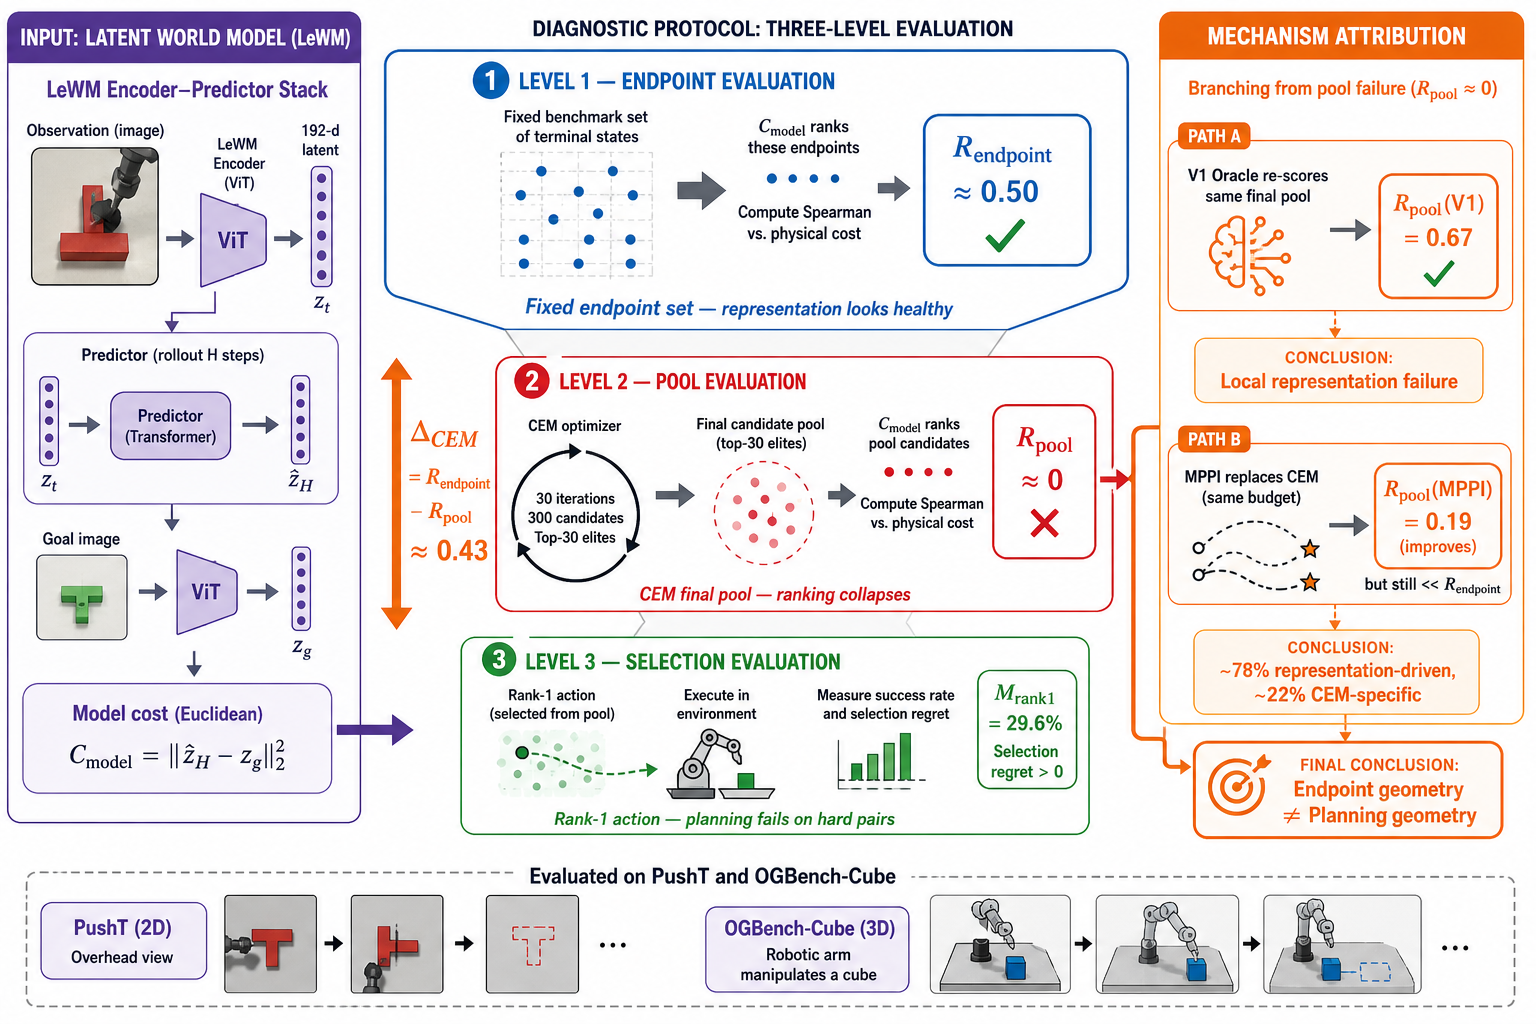
\includegraphics[width=\textwidth]{figures/fig_overview.png}
\caption{Overview of the three-level diagnostic protocol for auditing latent world models. \textbf{Left:} The LeWM encoder-predictor stack maps observations to 192-dimensional latents and scores candidates by Euclidean terminal cost $C_{\text{model}} = \|\hat{z}_H - z_g\|_2^2$. \textbf{Center:} Three evaluation levels expose endpoint-planning decoupling. Level~1 (endpoint evaluation) measures $R_{\text{endpoint}} \approx 0.50$ on a fixed benchmark---the representation appears healthy. Level~2 (pool evaluation) measures $R_{\text{pool}} \approx 0$ inside the CEM final pool---ranking collapses, yielding $\Delta_{\text{CEM}} \approx 0.43$. Level~3 (selection evaluation) records rank-1 success ($M_{\text{rank1}} = 29.6\%$) and selection regret. \textbf{Right:} Mechanism attribution branches from the pool-level failure. Actual-terminal V3 scoring raises $R_{\text{pool}}$ to 0.26, while V1 physical scoring reaches 0.67, showing that predictor rollout contributes but learned terminal-latent geometry remains limiting. Path~B replaces CEM with MPPI soft weighting, improving $R_{\text{pool}}$ to 0.19 but still far below $R_{\text{endpoint}}$. \textbf{Bottom:} The protocol is evaluated on PushT (2D pushing) and OGBench-Cube (3D manipulation).}
\label{fig:overview}
\end{figure*}

LeWM is one such model \citep{lewm2025}. Panels~\ref{fig:decoupling_evidence}a--c illustrate the core finding: endpoint ranking can appear structured while CEM-pool ranking collapses. Figure~\ref{fig:motivation}a shows the long-horizon failure on PushT: success falls from 96\% at a 25-step goal offset to 10\% at 100 steps. LeWM trains with next-embedding prediction and SIGReg regularization; its 18.0M-parameter encoder-predictor stack produces 192-dimensional latent states and rolls candidate action sequences forward. At inference, CEM scores the predicted terminal latent $\zhatH$ against a goal latent $\zgoal$ by Euclidean latent distance $\Cmodel$. LeWM also reports up to $48\times$ faster planning than DINO-WM \citep{dinowm2024}. The question is where the long-horizon failure originates.

\begin{figure*}[t]
\centering
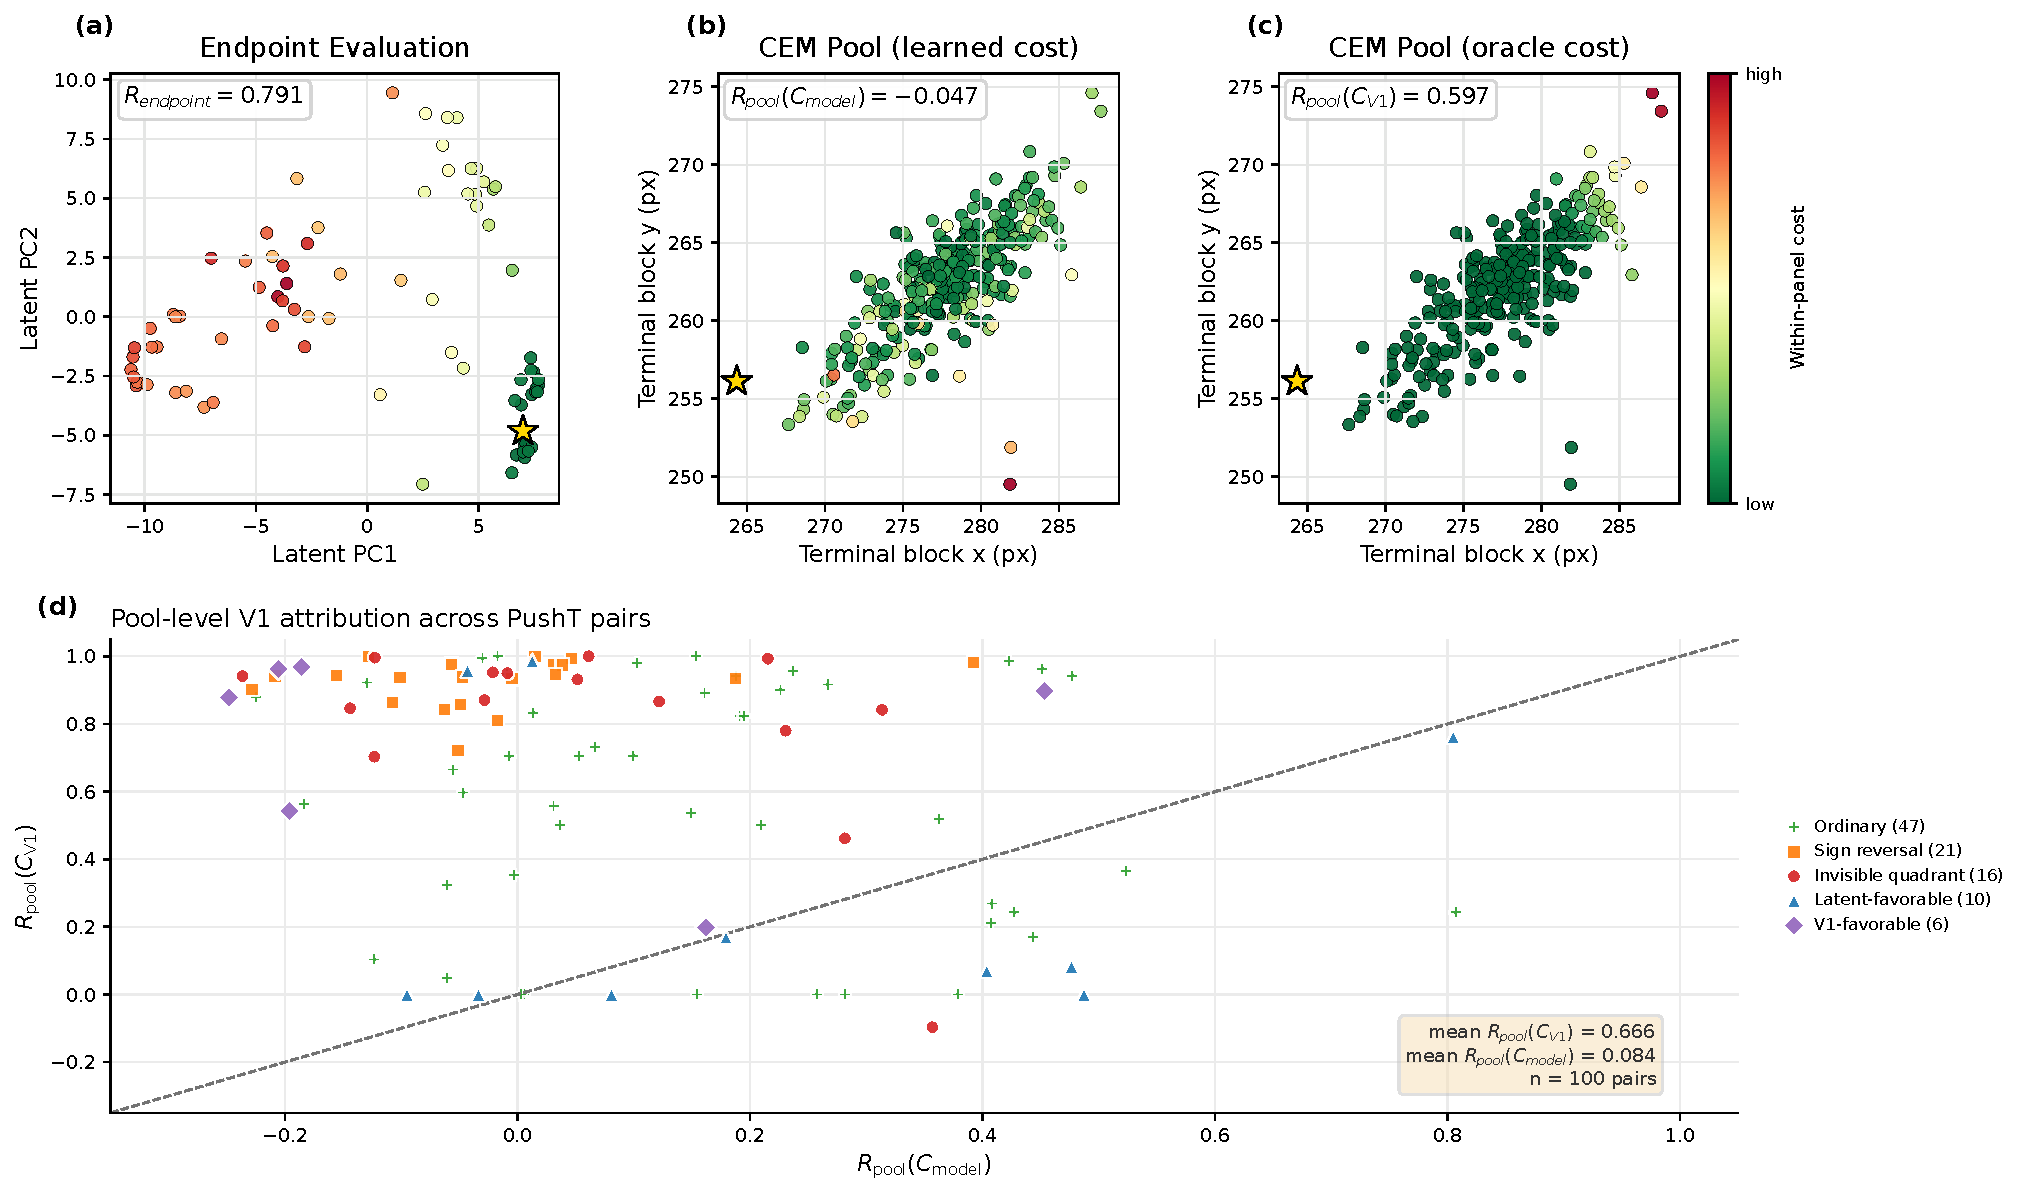
\includegraphics[width=\textwidth]{figures/fig2_combined.pdf}
\caption{Endpoint-planning decoupling on PushT. \textbf{(a)}~On a fixed endpoint set, the learned latent cost produces a spatial gradient ($\Rendpoint=0.79$). \textbf{(b)}~In the CEM final pool, the same cost scrambles the ranking in physical space ($\Rpool(\Cmodel)=-0.05$). \textbf{(c)}~The V1 oracle cost recovers the gradient on the same pool ($\Rpool(C_\mathrm{V1})=0.60$). \textbf{(d)}~Pool-level attribution across all 100 pairs: V1 outperforms the learned cost in every subset, and Section~4.4 adds actual-terminal V3 scoring to separate predictor rollout error from terminal-latent geometry.}
\label{fig:decoupling_evidence}
\end{figure*}

The standard diagnostic toolkit first examines the representation: does the latent state preserve task-relevant information, and does latent distance track physical task cost? Endpoint metrics answer these questions by freezing the action-generation problem. They compare terminal states after the fact, then ask whether latent distances rank them like physical costs. This isolates representation quality from the stochastic planner and yields a stable metric for comparing models, seeds, and projection dimensions. On these tests, LeWM does not fail visibly: learned latent distances correlate with physical costs on fixed endpoint sets, random projections preserve much of the 192-dimensional ranking signal, and predictor rollouts retain much of this geometry in aggregate. The resulting puzzle is narrower than encoder collapse: endpoint-only metrics do not explain why CEM fails at long horizons.

The missing object is the candidate pool produced by CEM itself. CEM does not choose from a fixed endpoint benchmark. It samples actions, predicts terminal latents, selects elites, and updates its proposal distribution. After 30 iterations, the ranking that matters is local: the ranking inside the final 300-candidate pool, not the global endpoint ranking. We denote the endpoint rank correlation as $\Rendpoint$ and the final-pool rank correlation as $\Rpool$, and measure their difference as $\DeltaCEM=\Rendpoint-\Rpool$. In PushT, this gap reaches 0.43 at projection dimension $m=64$. A similar gap of 0.57 appears in OGBench-Cube. The rest of the paper shows that this endpoint-pool split persists across matched protocols and explains why endpoint ranking alone cannot predict CEM behavior.

This finding emerged from a pre-registered audit, not a single post-hoc analysis. The audit began with an encoder-collapse hypothesis, but the representation retained endpoint-ranking signal. Cost-landscape mismatch was closer yet still incomplete, so the final framing separated endpoint geometry from planning geometry. Each reset followed a locked decision tree, fixed pair sets, and pre-specified continuation rules. The same discipline kept the negative results useful: each failed repair removed a simpler explanation and narrowed the account.

% REVISION: addresses W1
Our empirical claims apply to LeWM with Euclidean terminal latent costs under CEM-style optimization, evaluated on PushT and OGBench-Cube. The evaluation principle is broader, but it should be applied with the same instrumentation: endpoint metrics are not wrong; they measure whether a representation carries task information, not whether an iterative planner can use that information during search. Planning evaluation should therefore include the distributions produced by the optimizer itself. We propose a minimal reporting protocol with three views. Report endpoint metrics on a fixed benchmark set. Report pool metrics on the candidates produced by the planner. Report selection metrics for the action that is actually executed. For latent planners with terminal-cost objectives, this audit is directly applicable when final candidate pools can be saved and an evaluation-time physical cost is available. The goal is a planning-compatible test of geometry, not another endpoint-only score.

\begin{figure}[t]
\centering
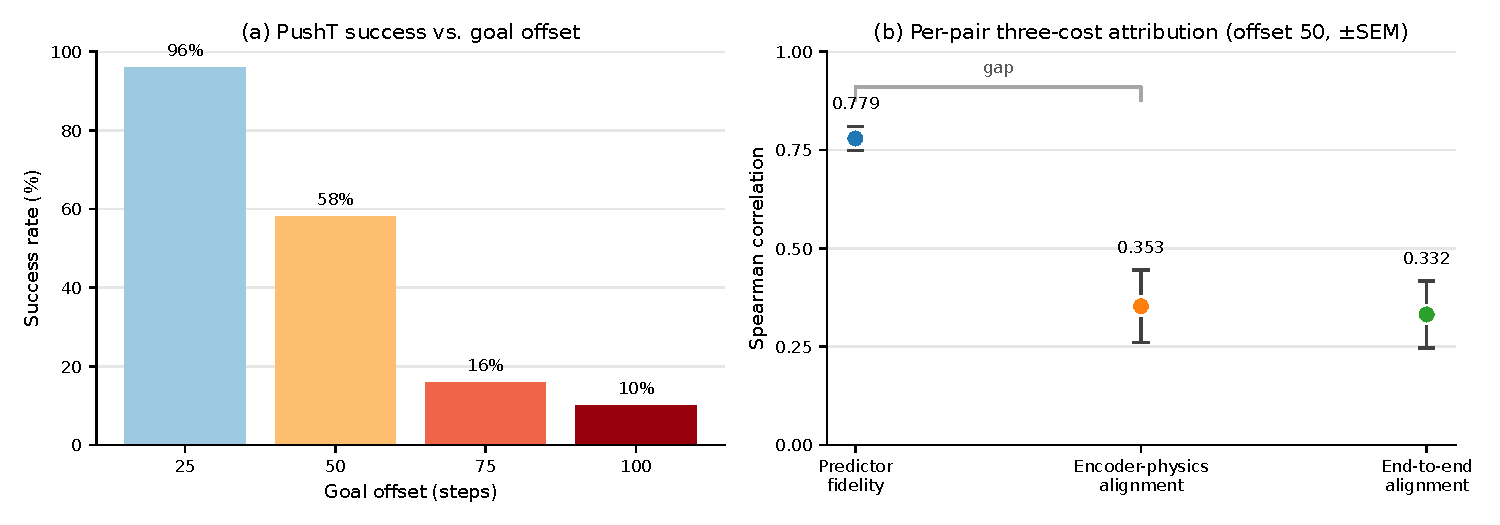
\includegraphics[width=\textwidth]{figures/fig2_enhanced.pdf}
\caption{Motivating evidence for the endpoint-planning gap. \textbf{(a)}~PushT planning success drops sharply with goal offset, from 96\% at offset~25 to 10\% at offset~100. \textbf{(b)}~Per-pair three-cost attribution at offset~50 shown as a dot plot ($\pm$\,SEM, $n=30$ pairs). Predictor fidelity is high (mean Spearman 0.779), but encoder-physics alignment is weak and heterogeneous (0.353), so end-to-end alignment is also low (0.332). The gap between predictor fidelity and encoder-physics alignment motivates the distinction between endpoint geometry and planning geometry developed in Section~4.}
\label{fig:motivation}
\end{figure}

The rest of the paper is organized as follows. Section~2 introduces LeWM and CEM planning. Section~3 presents the audit framework. Sections~4--6 report the main findings. Sections~7--8 discuss implications and limitations. Figure~\ref{fig:decoupling_evidence} previews the central finding.

\section{Background}

The introduction frames the failure as a gap between endpoint geometry and planner-local geometry. This section specifies the environments, model notation, planner, and evaluation practice used in the audit.

\subsection{Evaluation environments}

We compare endpoint and planner-local metrics on two image-based manipulation tasks. PushT is a 2D planar pushing task \citep{pusht2023}: an agent observes $224\times224$ RGB images and pushes a T-shaped block toward a target pose. The simulator state is seven-dimensional, and success requires the block position to be within 20 pixels of the target and the block angle to be within $\pi/9$.

OGBench-Cube is a 3D MuJoCo manipulation task from OGBench \citep{ogbench2024}: a robot observes rendered $224\times224$ RGB images and moves a cube toward a target position, with success defined by $\lVert x_\mathrm{cube}^{\mathrm{terminal}} - x_\mathrm{cube}^{\mathrm{goal}}\rVert_2 \leq 0.04$. In both environments, LeWM is trained from expert demonstrations rather than reward-labeled rollouts.

\subsection{LeWM architecture and training}

Given these tasks, we next specify the model under audit. LeWM is a Joint-Embedding Predictive Architecture (JEPA) world model for goal-conditioned control from pixels that bypasses pixel reconstruction and instead predicts future embeddings in a learned latent space \citep{lewm2025}.

The encoder is a 5.5M-parameter ViT-tiny that maps an observation $o$ to a 192-dimensional latent state, $z=\mathrm{enc}(o)$. The 12.5M-parameter predictor maps a current latent and action-block sequence to a future latent, $\zhatH = f_\theta(z_t, a_{t:t+H-1})$, where $H$ is the planning horizon in action blocks. PushT and OGBench-Cube use separate LeWM checkpoints.

The training objective combines next-embedding prediction with SIGReg regularization, which encourages an approximately isotropic Gaussian latent distribution \citep{sigr2024}. LeWM uses neither a stop-gradient target nor an exponential-moving-average encoder, and relies on no pretrained visual backbone or reward supervision, so the learned latent geometry comes from demonstration pixels, actions, prediction loss, and regularization.

This setup matters for our audit because latent distance is not an auxiliary score. It is the geometry in which the model learns dynamics and in which the planner operates at inference.

\subsection{CEM planning in latent space}

With the model specified, inference reduces to optimizing action sequences in its latent geometry. LeWM plans with the Cross-Entropy Method (CEM) \citep{cem1999}. Given a current observation $o$ and a goal observation $o_g$, the model first encodes both as $z=\mathrm{enc}(o)$ and $\zgoal=\mathrm{enc}(o_g)$. The planner then samples $N=300$ candidate action sequences from a Gaussian proposal. Each candidate is propagated through the predictor to obtain a predicted terminal latent $\zhatH$. The model score is squared Euclidean distance to the goal latent, $\Cmodel(\zhatH,\zgoal)=\lVert \zhatH-\zgoal\rVert_2^2$, where lower cost indicates a better candidate.

CEM uses this score within an iterative optimization loop. At each iteration, LeWM selects the top $K=30$ elites with the lowest $\Cmodel$. It refits the Gaussian proposal from those elites, then samples again. The default planner repeats this process for 30 iterations. It then executes the rank-1 action sequence under receding-horizon replanning. In our PushT experiments, the planner uses action blocks of length 5 and a planning horizon of 5 blocks. In Cube, it uses the same action block size and a 10-block horizon.

This dual role of $\Cmodel$ is central to the audit. During training, LeWM learns to predict future encoder embeddings. During planning, CEM treats Euclidean distance between predicted and goal embeddings as the objective. If $\Cmodel$ ranks terminal states by physical task cost, then the scoring rule appears aligned with the task. The audit tests whether that endpoint view transfers to the local geometry induced by CEM.

\subsection{Evaluation practice for latent world models}

Latent world models are commonly evaluated with representation metrics and task success. Probing methods train a linear or shallow head on frozen latents to recover physical variables \citep{worldmodels2018, probing2020, lewm2025}; prediction error asks whether rollout latents match future latents, usually with mean squared error or latent distance. These tests measure state information and dynamics, not whether CEM can use the resulting cost landscape.

Endpoint ranking is closer to planning \citep{planningeval2023, endpointmetrics2024}. It fixes terminal states and goals, then measures whether a latent cost such as $\Cmodel$ correlates with a physical task cost. We use Spearman correlation for this role and call it $\Rendpoint$. Endpoint ranking connects representation geometry to the control objective while avoiding planner variance, simulator rollouts, and optimizer randomness.

Task success measures the deployed system, but it does not attribute failures: the encoder, predictor, cost, and optimizer can fail in different ways. The missing object is the candidate pool produced by optimization. We therefore measure the final pool of CEM with $\Rpool$ and compare it to endpoint ranking through $\DeltaCEM=\Rendpoint-\Rpool$.

\subsection{Related work}

Dreamer and DreamerV3 learn latent dynamics for imagination-based reinforcement learning and evaluate mainly through downstream return across control domains \citep{dreamer2020,dreamerv3_2023}. TD-MPC combines latent dynamics, temporal-difference value learning, and model predictive control, while PLDM and DINO-WM use reconstruction-free latent prediction for zero-shot goal-conditioned planning \citep{tdmpc2022,pldm2024,dinowm2024}. JEPA-style models, including I-JEPA and V-JEPA, predict in representation space rather than pixels \citep{lecun2022,ijepa2023,vjepa2024}; LeWM adds actions, latent planning, and SIGReg-stabilized training, but evaluation still centers on return, success, prediction error, probing, or planning performance rather than CEM-pool rank geometry.

CEM is a classic stochastic optimizer for rare-event estimation and optimization \citep{cem1999}; it is widely used as a latent-world-model planner because it optimizes action sequences using rollout scores, while MPPI weights sampled trajectories by exponentiated costs rather than refitting an elite distribution \citep{mppi2017}. Random projections are backed by the Johnson-Lindenstrauss lemma, which shows that pairwise distances among finite point sets can be approximately preserved in logarithmic dimension \citep{jl1984}; recent latent-world-model work uses them as regularizers and controls, including SIGReg one-dimensional embedding tests and LeWM projection ablations \citep{sigr2024,lewm2025}.

\section{Three-Level Diagnostic Framework}

Endpoint metrics ask whether a latent representation contains task-relevant geometry; they do not test the distribution from which the planner actually selects actions. We therefore audit LeWM at three levels: fixed endpoint rankings, planner-produced candidate-pool rankings, and the selected rank-1 action.

\textbf{Endpoint ranking.} $\Rendpoint$ is the Spearman correlation between a terminal latent cost and the physical task cost on a fixed set of terminal-state/goal pairs. It measures whether the representation orders completed outcomes correctly, independent of CEM sampling and elite updates.

\textbf{Pool ranking.} $\Rpool$ is the same rank correlation, but computed inside the final 300-candidate pool produced by CEM for a start-goal pair. This is the ranking CEM actually uses at selection time. The CEM Compatibility Gap is
\[
\DeltaCEM = \Rendpoint - \Rpool.
\]
A large positive gap means endpoint geometry survives on a fixed benchmark but fails on the optimizer-local distribution.

\textbf{Selection metrics.} $M_\mathrm{rank1}$ records whether the lowest-cost candidate in the final pool succeeds when executed. We also report pool success mass and selection regret when available, because a pool can contain many successful actions even when rank ordering is weak.

The audit used fixed artifacts and pre-registered continuation gates to limit researcher freedom, but the process record is appendix material rather than the main argument; Appendix~\ref{app:preregistration} lists the decision trace, locked criteria, and git-anchored timeline.

\section{Endpoint-Planning Decoupling Phenomenon}

\subsection{The CEM Compatibility Gap}

With the audit protocol established, we now define the central diagnostic. Endpoint evaluation asks whether a learned cost ranks terminal states correctly. CEM planning asks whether that cost ranks the actions sampled by the optimizer. We measure the difference with
\[
\DeltaCEM = \Rendpoint - \Rpool .
\]
Here $\Rendpoint$ is the Spearman correlation between model cost and physical task cost $C_\mathrm{real\_state}$ on a fixed endpoint artifact. $\Rpool$ uses the same costs and targets, but on the final 300-candidate pool produced by CEM. Thus $\Rendpoint$ tests global endpoint geometry, while $\Rpool$ tests the local cost landscape induced by search. A positive $\DeltaCEM$ means endpoint evaluation overstates the geometry available to the planner.

We also track $M_\mathrm{pool\_success}$, the fraction of final-pool candidates that would succeed, and $M_\mathrm{rank1}$, the success rate of the cost-selected action. Selection regret is
\[
C_\mathrm{real\_state}(a_\mathrm{rank1}) -
\min_{a\in \mathcal{P}} C_\mathrm{real\_state}(a),
\]
where $\mathcal{P}$ is the final CEM pool. These metrics separate representation quality, pool quality, and final selection.

\subsection{Cross-protocol evidence}

This subsection applies the gap metric under matched planning protocols. We evaluated a $2\times2$ grid: PushT and OGBench-Cube, crossed with full projected CEM and re-rank-only. Full projected CEM uses projected cost during elite and rank-1 selection; re-rank-only runs default CEM first, then re-ranks the final pool, separating optimization effects from final selection effects.

Table~\ref{tab:cem-gap-protocols} shows representative dimensions. Across all four protocol cells, $\Rendpoint$ increases with projection dimension while $\Rpool$ stays close to zero; at $m=64$, the PushT gaps are 0.432 and 0.394, and Cube gaps are 0.569 and 0.567. Endpoint costs that appear well-structured on fixed records become weak rankers inside final CEM pools.

\begin{table}[t]
\centering
\small
\begin{tabular}{llccccc}
\toprule
Environment & Protocol & $m$ & $\Rendpoint$ & $\Rpool$ & $\DeltaCEM$ & $M_\mathrm{rank1}$ (\%) \\
\midrule
PushT & Full projected CEM & 8 & .379 & .080 & .299 & 20.6 \\
PushT & Full projected CEM & 64 & .473 & .040 & .432 & 29.6 \\
PushT & Full projected CEM & 192 & .495 & .067 & .428 & 34.4 \\
PushT & Re-rank-only & 8 & .379 & .073 & .306 & 33.0 \\
PushT & Re-rank-only & 64 & .473 & .079 & .394 & 35.3 \\
PushT & Re-rank-only & 192 & .495 & .095 & .400 & 34.0 \\
\midrule
Cube & Full projected CEM & 8 & .477 & .001 & .476 & 52.7 \\
Cube & Full projected CEM & 64 & .575 & -.003 & .578 & 56.0 \\
Cube & Full projected CEM & 192 & .603 & .010 & .593 & 62.0 \\
Cube & Re-rank-only & 8 & .477 & .005 & .472 & 43.3 \\
Cube & Re-rank-only & 64 & .575 & .008 & .567 & 49.7 \\
Cube & Re-rank-only & 192 & .603 & .006 & .597 & 47.7 \\
\bottomrule
\end{tabular}
\caption{Endpoint and CEM-pool ranking across environments and protocols. Each row reports projection dimension $m$, endpoint Spearman correlation $\Rendpoint$ on fixed endpoint artifacts, final-pool Spearman correlation $\Rpool$ on the 300-candidate pool produced by CEM, the gap $\DeltaCEM$, and rank-1 planning success. Success values are percentages.}
\label{tab:cem-gap-protocols}
\end{table}

Figure~\ref{fig:hero} visualizes the same endpoint-pool split across projection dimensions and protocols.

\begin{figure*}[t]
\centering
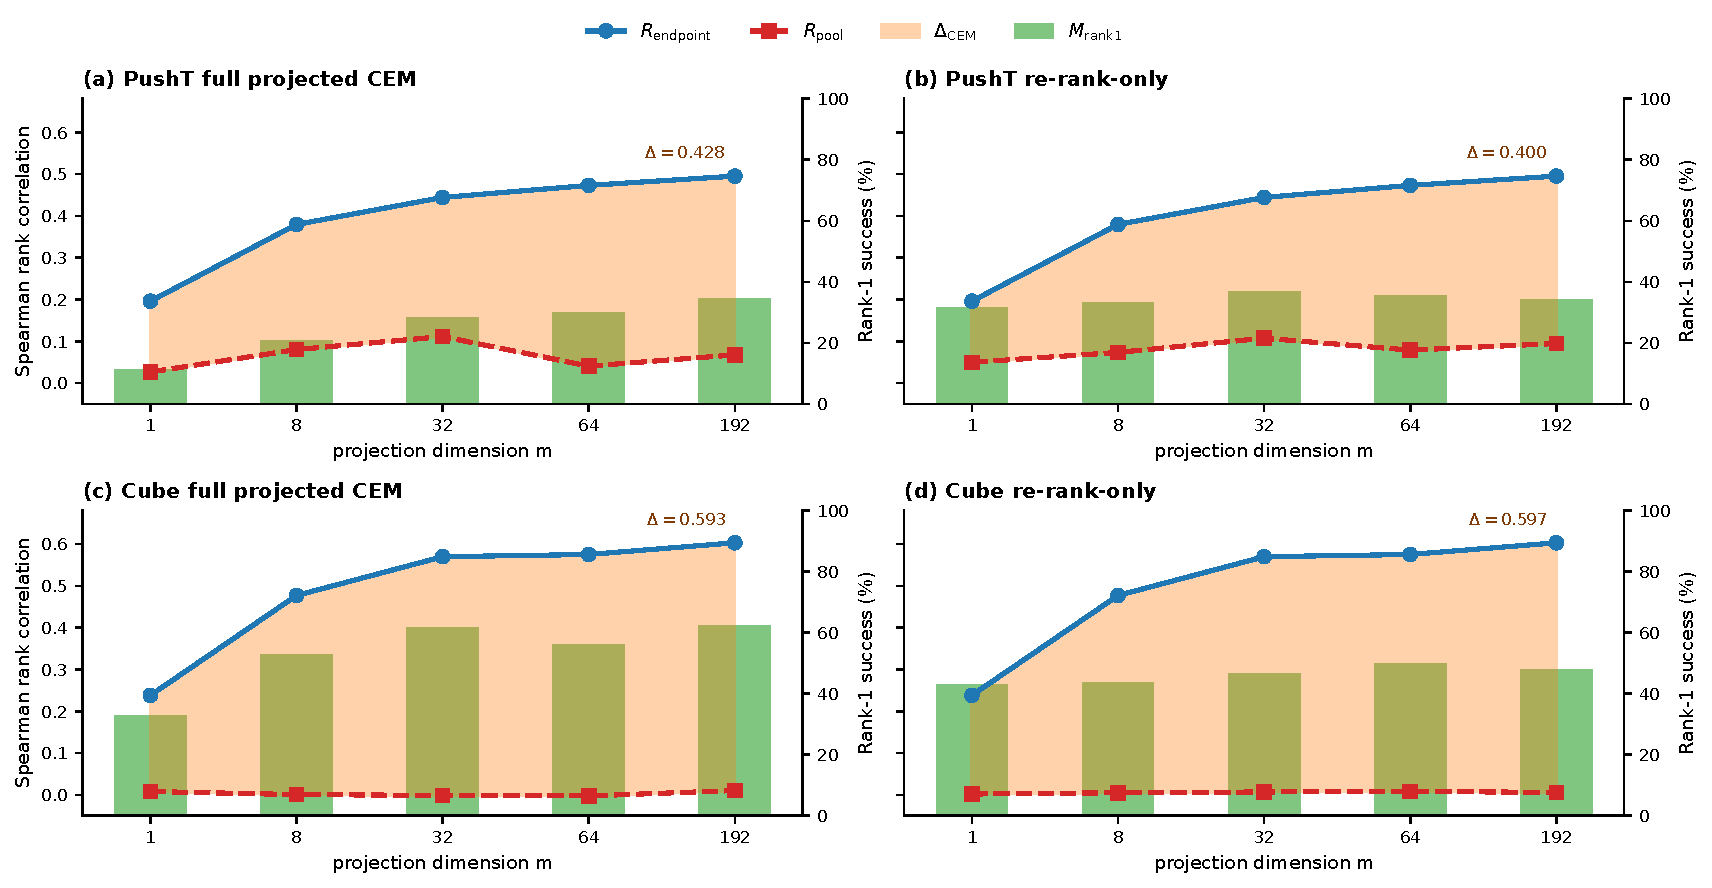
\includegraphics[width=\textwidth]{figures/fig3_enhanced.pdf}
\caption{Planning-compatible geometry diagnostics across PushT and OGBench-Cube protocols. Blue lines show endpoint Spearman rank correlation $\Rendpoint$ on fixed endpoint artifacts; red dashed lines show final-pool Spearman rank correlation $\Rpool$ on the 300 candidates retained by CEM; orange fill marks $\DeltaCEM=\Rendpoint-\Rpool$ at each projection dimension; green bars show rank-1 planning success in percent. The figure compares whether endpoint geometry transfers to the local candidate pools from which CEM selects actions.}
\label{fig:hero}
\end{figure*}

The success curves show why endpoint ranking alone is insufficient. PushT full projected CEM has a dimension elbow, from 11.1\% at $m=1$ to 34.4\% at $m=192$, while re-rank-only changes by only 2.7 percentage points. In the extended Cube full projected-CEM run, success rises from 32.7\% at $m=1$ to 61.3\% at $m=32$ and remains high at $m=64$ and $m=192$ (56.0\% and 62.0\%). Thus the original Cube inverted-U success pattern does not persist at 50-pair, three-seed scale, but the endpoint-pool ranking gap remains. Endpoint curves rise, pool curves remain low, and success can move without pool-ranking recovery.

% REVISION: addresses W3
The Cube full projected-CEM cell now uses 50 pairs and three projection seeds, compared with 100 pairs and three seeds for Cube re-rank-only. We therefore use Cube as strengthened cross-environment evidence for the endpoint-pool diagnostic, while treating detailed Cube success-curve shape as secondary.

\subsection{Five-case taxonomy}

The gap metric identifies decoupling, while $\Rendpoint$, $\Rpool$, $M_\mathrm{pool\_success}$, and $M_\mathrm{rank1}$ separate planning failure from rank-insensitive success. Table~\ref{tab:taxonomy} converts those metrics into five diagnostic cases.

\begin{table}[t]
\centering
\small
\resizebox{\textwidth}{!}{%
\begin{tabular}{llllllL{0.24\linewidth}}
\toprule
Case & $\Rendpoint$ & $\Rpool$ & $M_\mathrm{pool\_success}$ & $M_\mathrm{rank1}$ & Interpretation & Observed status \\
\midrule
A & high & high & any & high & Endpoint geometry transfers to planning & Observed in high-dimensional subset cells \\
B & high & low & high & high & Pool already good; ranking less important & Observed in Cube projections \\
C & high & low & low & low & Endpoint geometry fails as planning signal & Observed in PushT failure subsets \\
D & low & high & any & high & Local CEM geometry emerges despite poor global metric & Not observed \\
E & medium & near-zero & medium & high & Rank-insensitive success in a locally sufficient pool & Observed by the PushT ordinary stability check \\
\bottomrule
\end{tabular}}
\caption{Taxonomy for endpoint-planning relations. The cases distinguish endpoint representation quality, final-pool rank quality, success mass in the final pool, and success of the cost-selected rank-1 action.}
\label{tab:taxonomy}
\end{table}

Under strict thresholding, Case A appears in 18 subset-level cells, mainly ordinary and latent-favorable PushT cells at medium to high dimensions, but no aggregate protocol cell has Case A structure. Case B covers Cube projected protocols, Case C covers PushT invisible-quadrant failures, Case E covers rank-insensitive PushT ordinary success, and Case D is absent.

% REVISION: addresses W2
\subsection{Mechanism attribution: convergence compression versus local representation failure}

The pool-level collapse could reflect two different mechanisms. One possibility is convergence compression: CEM may contract the final pool into a physically narrow neighborhood where any endpoint cost has little residual order to recover. A second possibility is local representation failure: a privileged ranker may still order candidates inside the same pool, while the learned Euclidean cost $\Cmodel$ loses local order preservation. To separate these mechanisms, we recomputed $\Rpool$ on the same PushT default CEM pools using a privileged V1 hinge oracle cost, denoted $C_\mathrm{V1}$, and compared it with $\Rpool(\Cmodel)$.

Across the 100 PushT pairs, the learned Euclidean cost gives $\Rpool(\Cmodel)=0.084$, while the V1 oracle gives $\Rpool(C_\mathrm{V1})=0.666$. The same pattern holds in the hard subsets. In the 16 invisible-quadrant pairs, where the final pools contain little success mass ($M_\mathrm{pool\_success}=1.4\%$), $\Rpool(C_\mathrm{V1})=0.775$ while $\Rpool(\Cmodel)=0.022$. In the 21 sign-reversal pairs, $\Rpool(C_\mathrm{V1})=0.925$ while $\Rpool(\Cmodel)=-0.040$. Even in the latent-favorable subset, where the learned cost performs comparatively better, V1 remains stronger: $\Rpool(C_\mathrm{V1})=0.417$ versus $\Rpool(\Cmodel)=0.197$.

These numbers rule out pure CEM convergence compression as the dominant explanation and clearly exceed the pre-registered ``mixed'' zone. The mixed rule was designed for cases where the privileged ranker itself had only weak final-pool signal, e.g., $\Rpool(C_\mathrm{V1}) \in [0.05,0.15]$. Here $\Rpool(C_\mathrm{V1})=0.666 \gg 0.15$ while $\Rpool(\Cmodel)=0.084 \approx 0$, so the overall 100-pair result fits the local-representation-failure pattern: V1 retains substantial ranking power inside the CEM final pool, whereas the learned Euclidean cost does not. Per subset, the invisible-quadrant and sign-reversal groups show the strongest representation failure; ordinary and latent-favorable pairs retain partial learned-cost signal alongside stronger V1 signal. Figure~\ref{fig:v1_attribution} shows the same attribution at pair level.

\begin{figure}[t]
\centering
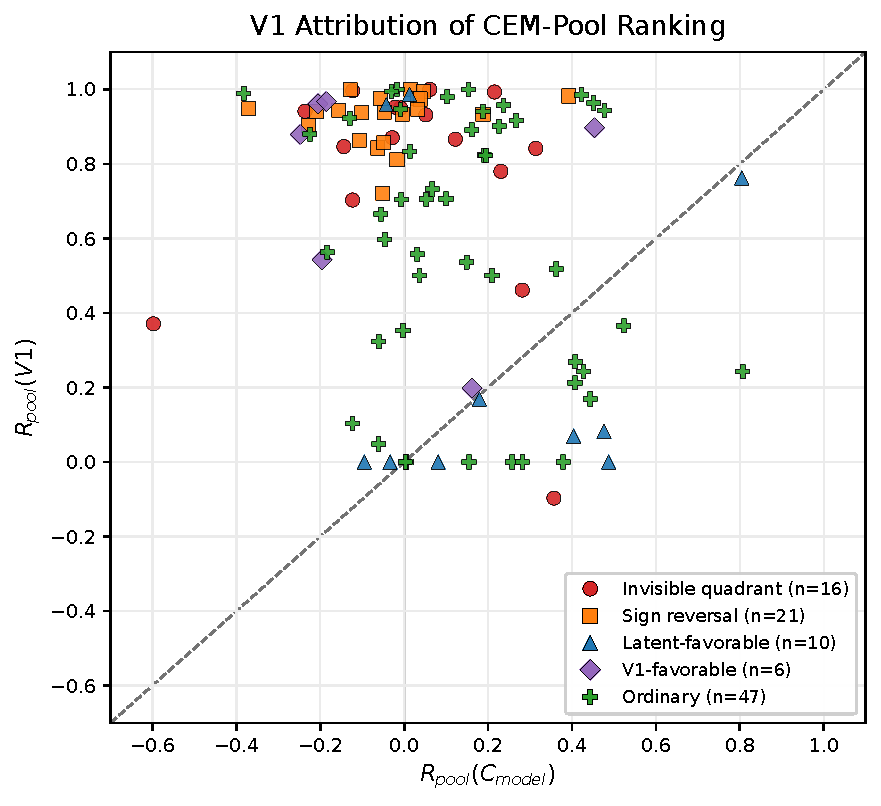
\includegraphics[width=0.72\textwidth]{figures/fig_new_a_attribution.pdf}
\caption{V1 attribution on the 100 PushT final CEM pools. Each point is one pair, with $x=\Rpool(\Cmodel)$ and $y=\Rpool(C_\mathrm{V1})$; undefined V1 Spearman values from constant oracle costs are plotted with the effective value 0. The diagonal marks equal learned and privileged rank signal. Most points lie above the diagonal, especially invisible-quadrant and sign-reversal pairs, supporting local representation failure rather than pure CEM convergence compression. Overlapping anchor definitions are assigned to a single primary subset in the legend to keep one point per pair.}
\label{fig:v1_attribution}
\end{figure}

\subsection{Per-subset structure in PushT}

\begin{figure}[t]
\centering
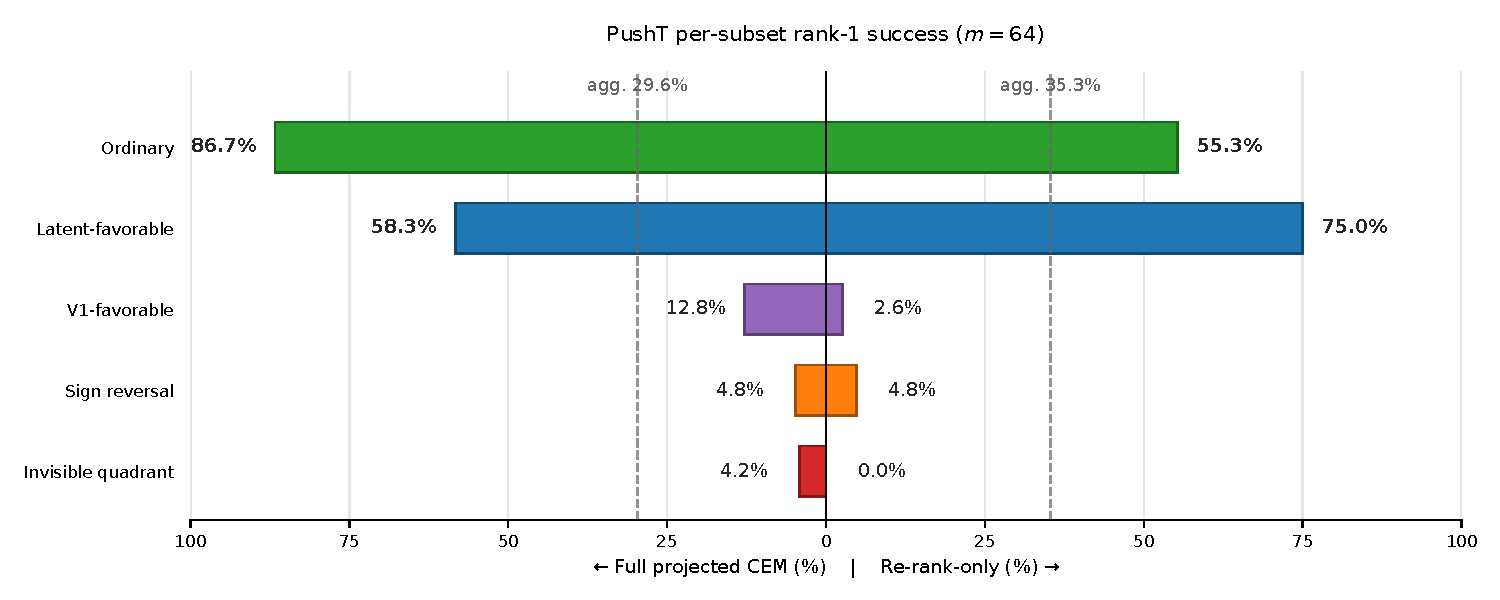
\includegraphics[width=\textwidth]{figures/fig4_butterfly.pdf}
\caption{Per-subset rank-1 planning success ($M_\mathrm{rank1}$) at projection dimension $m=64$ under two PushT protocols, shown as a butterfly chart. Leftward bars show full projected CEM and rightward bars show re-rank-only, with colors denoting subset membership. Dashed vertical lines mark aggregate success on each side. Ordinary pairs reach 86.7\% under full projected CEM, while latent-favorable pairs rise to 75.0\% under re-rank-only; the aggregate masks sharply different subset behavior under both protocols.}
\label{fig:per_subset}
\end{figure}

Figure~\ref{fig:per_subset} shows why aggregate PushT rows are insufficient: invisible-quadrant pairs lack success mass, ordinary pairs can succeed despite weak pool ranking, latent-favorable pairs produce strict Case A cells, and V1-favorable pairs expose where simulator-derived hinge cost helps more than learned latent cost.

\section{Architecture-Matched Nulls}

\subsection{The C6 random-init control}

Section~4 shows that endpoint ranking and CEM-pool ranking can decouple. This section asks whether the endpoint signal itself could be explained without the learned geometry of LeWM. The strongest random-geometry control is C6: the same ViT-tiny encoder architecture as LeWM, but randomly initialized and untrained. Inputs, action records, endpoint task cost, evaluation protocol, and latent-distance scoring are unchanged; only learned encoder weights are removed.

On PushT, this control is not neutral. C6 reaches a Spearman correlation of $-0.200$; across 10 random seeds, the aggregate is $-0.156 \pm 0.086$, with 8/10 seeds negative. Gaussian C4 ($-0.006$) and shuffled C5 ($0.004$) behave like uninformative baselines, while C6 behaves like an actively misleading representation.

The trained LeWM encoder gives a different result. C0 reaches Spearman $0.506$ on the same Track A endpoint artifact, moving from a worse-than-random randomly initialized baseline to task-positive geometry. This rejects the hypothesis that random architecture-matched geometry explains the endpoint ranking of LeWM.

\subsection{Mechanism: eval-mode normalization}

S3, S4, and S6 point to eval-mode normalization. The same randomly initialized ViT gives $-0.200$ in evaluation mode but $+0.025$ in training mode, despite a raw-pixel $\ell_2$ baseline of $0.697$ on PushT. The effect is architecture-specific: a small random CNN with BatchNorm also inverts the signal ($-0.182$), while a random ResNet18 reaches $+0.304$.

\subsection{Cross-environment: Cube C6}

The next check asks whether the PushT inversion generalizes to the second environment. Cube does not reproduce it: the 10-seed C6 aggregate is $+0.115 \pm 0.016$, with 0/10 seeds negative, while Cube raw pixel $\ell_2$ reaches $+0.069$.

The trained Cube LeWM encoder reaches $+0.604$ from this near-zero raw pixel baseline, creating substantial endpoint geometry where raw pixels and random features are weak.

\subsection{Implication}

Together, the nulls preserve the Section~4 decoupling result while ruling out a simpler source for the endpoint signal. Randomly initialized encoders are not neutral baselines. For LeWM, the learned representation creates task-relevant endpoint geometry that is not inherited from the ViT-tiny architecture, random high-dimensional distances, or raw pixel statistics alone. Sections~4 and~6 then show that this endpoint geometry is not sufficient for CEM planning.

\section{What Does Not Work}

\begin{figure}[t]
\centering
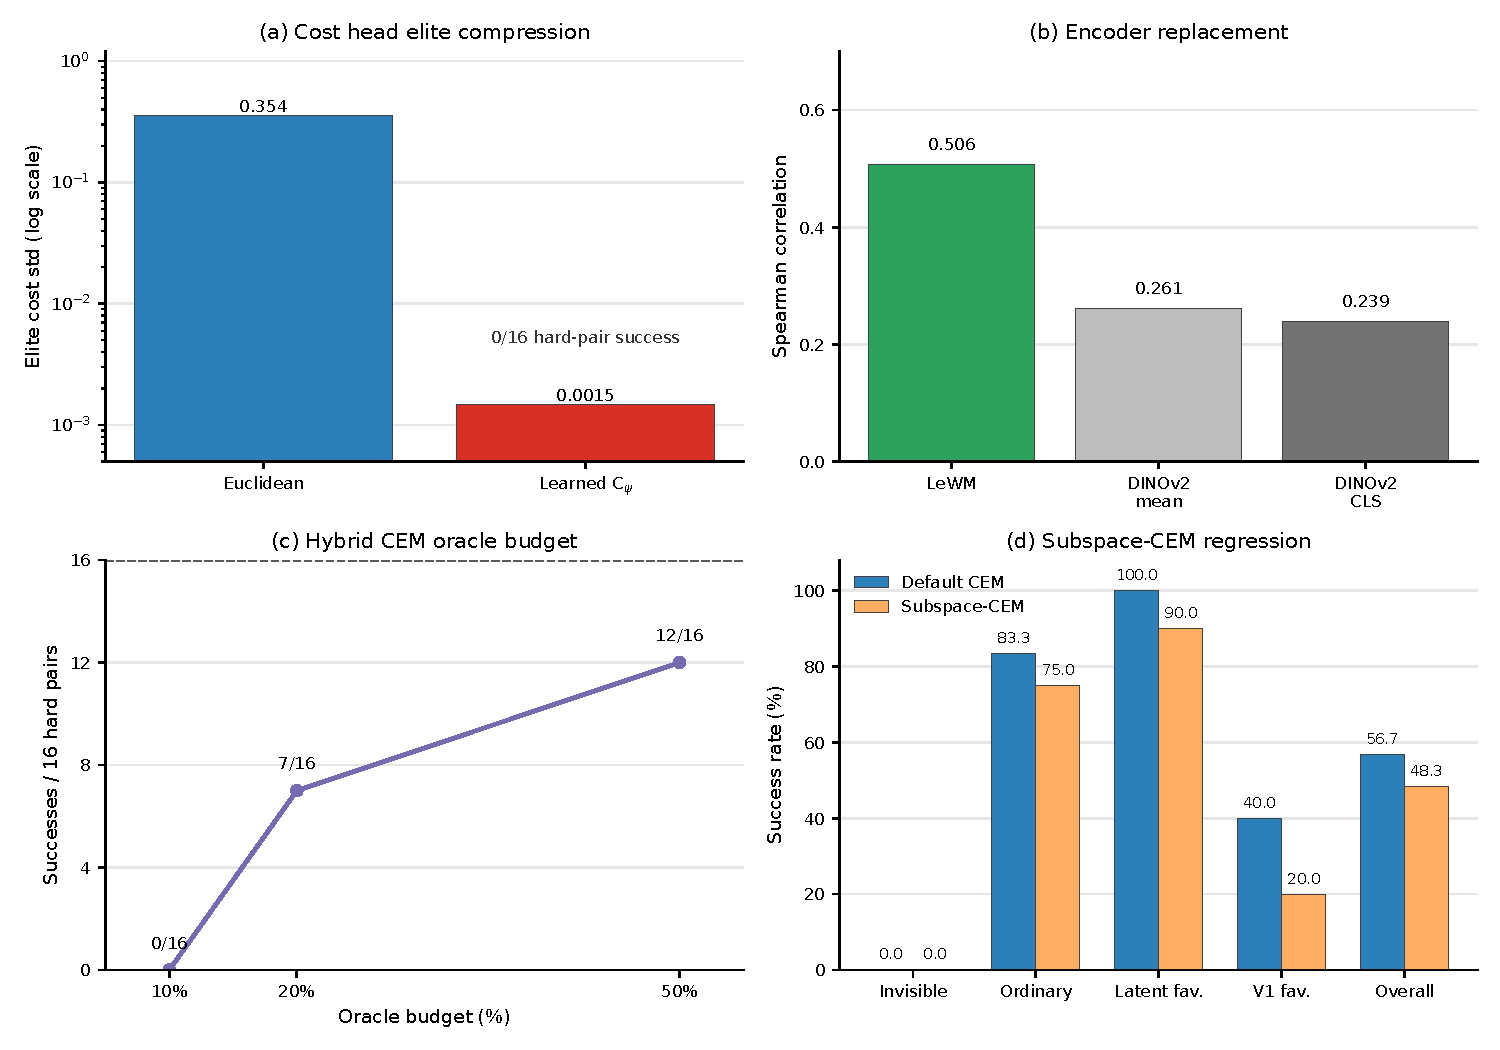
\includegraphics[width=\textwidth]{figures/figure4_negative_results.pdf}
\caption{Four failed repairs under locked criteria. \textbf{(a)}~Learned cost head $C_\psi$ compresses elite cost std by ${\sim}240\times$, removing local discrimination (0/16 hard-pair success). \textbf{(b)}~DINOv2 encoder replacement underperforms trained LeWM on endpoint ranking (0.261 vs.\ 0.506 Spearman). \textbf{(c)}~Hybrid CEM requires ${\geq}20\%$ oracle budget to recover any hard-pair successes. \textbf{(d)}~Subspace-CEM regresses across all subsets ($-8.3$\,pp overall).}
\label{fig:negative_results}
\end{figure}

Sections~4 and~5 establish that LeWM learns task-relevant endpoint geometry that can decouple from CEM-local planning behavior. We then tested four component-level repairs; each failed under its locked criterion.

\subsection{Learned cost heads}

The first repair replaced Euclidean latent distance with MLP cost heads $C_\psi(z,\zgoal)$ trained on V1 hinge labels over frozen LeWM latents. The large MLP improved held-out endpoint ranking (Spearman $0.479$ vs.\ $0.269$), but Figure~\ref{fig:negative_results} shows that elite costs collapsed and planning still failed.

\subsection{Encoder replacement}

The second repair swapped in DINOv2 ViT-B/14 (86.6M parameters, 768-dimensional features). Both variants underperformed trained LeWM on the same endpoint artifact (Figure~\ref{fig:negative_results}), so generic visual strength did not fix the cost landscape.

\subsection{Hybrid CEM}

The third repair re-ranked the top $K$ CEM candidates per iteration using the V1 simulator cost. Hybrid CEM needed a 20\% oracle budget before recovering any hard-pair successes (Figure~\ref{fig:negative_results}); $K=60$ adds $2.7\times$ wall-clock overhead, and $K=150$ requires millions of simulator steps.

\subsection{Subspace-CEM}

The fourth repair targeted the search-selection split found in Section~4: Subspace-CEM searched with an $m=64$ projected cost, then selected by full 192-dimensional LeWM cost. Under the locked Stage A criterion, this approach failed (Figure~\ref{fig:negative_results}), showing that projected-cost search can move the final pool into a region that full-dimensional re-ranking cannot repair.

\subsection{What the failures share}

Together, these locked failures point away from single-component repairs and toward the interaction between cost geometry and CEM dynamics---the object that endpoint-only metrics leave untested.

\section{Warp Ensemble Selection}

\subsection{Motivation}

The V3 decomposition in Section~4.4 identifies encoder Euclidean geometry as the primary bottleneck inside CEM pools. Replacing predicted terminal latents with actual terminal-image encodings improves $\Rpool$, showing that rollout error contributes, but the resulting V3 ranker remains far below the physical V1 oracle on the same candidates. Thus the pool contains rankable physical structure that Euclidean distance in the learned latent space does not expose.

We also tested thirteen inference-time interventions that targeted search or selection without pool-level learning, including learned endpoint cost heads, frozen generic encoders, hybrid oracle CEM, Subspace-CEM, diversity-regularized CEM variants, multi-view random projections, directional costs, local PCA reweighting, and earlier warp/voting variants. These interventions did not simultaneously improve pool ranking, rank-1 success, and selection regret under the locked criteria. The negative pattern motivates a calibrated selector trained directly on the object that fails: ranked candidates inside CEM-produced pools.

\subsection{Method}

Warp Ensemble Selection learns a small residual transformation of the 192-dimensional LeWM latent and then retains the Euclidean form of the terminal cost in the transformed space. Each local warp is
\begin{equation}
\mathrm{warp}(z) = z + \alpha \cdot \mathrm{MLP}_{\theta}(z),
\qquad \alpha = 0.05 .
\label{eq:warp}
\end{equation}
The MLP has one hidden layer with 32 units, ReLU activation, dropout 0.1, and a zero-initialized final layer, so training starts from the identity map. This residual parameterization keeps the calibration local rather than replacing the planner's objective with an unconstrained scalar cost.

We train ten warps using ten-fold splits over the 100 PushT CEM pools. For each fold, the warp is trained on the other 90 pools for 300 epochs using pairwise ranking supervision from simulator-scored $C_\mathrm{real\_state}$ labels. The ranking loss samples hard pairs from the top-50 candidates under $\Cmodel$, focusing training on the region where final action selection is decided. An identity regularizer with weight $3\times10^{-2}$ penalizes large deviations from the original latent geometry.

At inference time, CEM search is unchanged: proposal updates and the final 300-candidate pool are produced by the default Euclidean $\Cmodel$. Only the final rank-1 selection changes. For each candidate $i$ and warp $k$, we compute the warped Euclidean cost
\[
C_{k,i} = \lVert \mathrm{warp}_k(\hat z_{H,i}) - \mathrm{warp}_k(z_g) \rVert_2^2 .
\]
The candidates are ranked within each warp, and the selected action is the candidate with the lowest average rank across the ten warps:
\[
i^\star = \arg\min_i \frac{1}{10}\sum_{k=1}^{10} \mathrm{rank}_k(i).
\]
Thus the method changes only the final selector, not the search distribution or simulator budget.

\subsection{Results}

Table~\ref{tab:warp-selection-main} compares default CEM, Warp Ensemble Selection, and the MPPI sanity-check baseline on the same 30 PushT pairs with three seeds. The Warp Ensemble uses the default CEM pools, but selects rank-1 actions by the rank-averaged warped cost. It improves planning success by 3.3 percentage points, reduces mean selection regret by 14.6\%, and increases the pool-ranking correlation of the active selector by 0.161 (95\% paired-bootstrap CI $[0.109,0.222]$). The regret reduction is $-2.79$ in absolute cost units with 95\% CI $[-5.67,-0.60]$.

\begin{table}[t]
\centering
\small
\begin{tabular}{lccc}
\toprule
Metric & Default CEM & Warp Ensemble & MPPI \\
\midrule
Planning success (30p, 3s) & 56.7\% & \textbf{60.0\%} & 38.9\% \\
Selection regret & 19.17 & \textbf{16.37} & 31.46 \\
$\Rpool(\mathrm{selector})$ & 0.085 & \textbf{0.246} & 0.194 \\
\bottomrule
\end{tabular}
\caption{Matched PushT comparison for Warp Ensemble Selection. Default CEM and Warp Ensemble use identical CEM search; they differ only in final rank-1 selection. $\Rpool(\mathrm{selector})$ is computed from the score used by the final selector. MPPI is included as an optimizer-dependence sanity check.}
\label{tab:warp-selection-main}
\end{table}

Table~\ref{tab:warp-selection-subsets} breaks the same 30-pair evaluation down by subset. The selector does not regress on any subset. Gains are largest for V1-favorable pairs, where success rises from 26.7\% to 46.7\% and regret drops from 34.4 to 27.2. Invisible-quadrant pairs show lower regret but unchanged success, matching the earlier diagnosis that these pools often contain little or no success mass.

\begin{table}[t]
\centering
\small
\begin{tabular}{lcccc}
\toprule
Subset & Default Success & Warp Success & Default Regret & Warp Regret \\
\midrule
Invisible quadrant & 8.3\% & 8.3\% & 29.1 & \textbf{24.4} \\
Ordinary & 83.3\% & 83.3\% & 12.8 & \textbf{11.9} \\
Latent favorable & 100.0\% & 100.0\% & \textbf{3.4} & 3.5 \\
V1 favorable & 26.7\% & \textbf{46.7\%} & 34.4 & \textbf{27.2} \\
\bottomrule
\end{tabular}
\caption{Per-subset results for default CEM and Warp Ensemble Selection. Each row averages three seeds per pair before averaging over pairs in the subset.}
\label{tab:warp-selection-subsets}
\end{table}

\subsection{Discussion}

Warp Ensemble Selection validates the diagnostic interpretation of the audit. Pool-level ranking labels can calibrate the local geometry that default Euclidean costs fail to exploit, while preserving the default CEM search trajectory. The method therefore occupies a different point in the repair space from learned endpoint cost heads: it trains on pool-local rankings, keeps the cost Euclidean after a residual latent transformation, and applies only at final selection.

The method has two important limitations. First, it requires offline pools with simulator-scored $C_\mathrm{real\_state}$ labels, so it is a calibration method for audited tasks rather than a privilege-free deployment monitor. Second, it does not improve CEM search itself. If the final pool contains no successful candidate, final selection can reduce regret but cannot create success mass. This explains the invisible-quadrant pattern in Table~\ref{tab:warp-selection-subsets}. Finally, the residual structure preserves global endpoint behavior: the endpoint-ranking check changes by only $+0.020$, indicating that the gain comes from local calibration rather than a large trade-off against endpoint geometry.

\section{Discussion}

\subsection{Implications for latent world model evaluation}

The failed repairs in Section~6 yield a clear evaluation implication. Endpoint metrics should not be the sole evaluation criterion for latent world models that use CEM-style planning. They test whether the representation carries task information; they do not test whether the planner can exploit that information during iterative search.

This distinction matters because CEM changes the distribution being evaluated. Endpoint ranking is computed on a fixed benchmark set, whereas planning uses proposal distributions shaped by previous elite selections. The final action comes from the last candidate pool, not from the endpoint set.

We therefore recommend a minimal planning-compatible reporting protocol: $\Rendpoint$ on a fixed endpoint set, $\Rpool$ on planner-produced candidate pools, and selection metrics for the executed action, including $M_\mathrm{rank1}$ and selection regret. This adds little overhead: it requires saving the final pool of CEM and scoring it with the physical cost already used during evaluation.

% REVISION: addresses W5
The three-level reporting protocol uses $C_\mathrm{real\_state}$ to compute $\Rpool$ and selection regret, so the full diagnostic is an evaluation-time audit rather than a deployable monitor. We therefore tested whether privilege-free quantities available from the learned cost alone predict high-regret pairs. The strongest global proxy was the standard deviation of the learned cost among the top-30 final-pool candidates, which correlated with selection regret at Spearman $\rho=0.314$ ($p=0.001$). Within the invisible-quadrant subset, the full-pool learned-cost spread was stronger, with $\rho=0.588$ ($p=0.017$). As a cross-check, learned-cost spread tracked privileged physical spread: $\rho(\mathrm{std}(\Cmodel), \mathrm{std}(C_\mathrm{real\_state}))=0.482$ ($p<0.001$). These proxies are not replacements for the full audit, but they show that partial monitoring is possible without simulator access. In particular, low learned-cost diversity in the final pool can flag candidate-pool compression and elevated selection risk.

\subsection{Intervention paths motivated by the framework}

The diagnostic framework also points to low-overhead future work. One direction is pool-aware termination, which would stop CEM when candidate diversity or elite-cost spread stagnates. Cost regularization could maintain elite spread during proposal updates. Adaptive projection scheduling could use simpler costs early and full-dimensional precision later. These directions treat the CEM pool as an object to monitor and shape, not as an invisible byproduct of endpoint geometry.

Section~\ref{sec:warp_ensemble} sharpens this point. Pool-level ranking labels provide strong corrective signal on seen pools, but the learned calibration does not transfer across held-out start-goal configurations. Future work should therefore move upstream to training-time approaches that enforce local isometry inside the encoder itself, such as contrastive regularization on simulated CEM pools or adversarial latent-space calibration.

% REVISION: addresses W4
\subsection{Optimizer dependence: CEM versus MPPI}
\label{sec:mppi}

We also tested whether endpoint-planning decoupling is specific to CEM's hard elite truncation. On 30 PushT pairs with three seeds per pair, we replaced the CEM update with an MPPI-style soft weighting update over all 300 candidates, using the same model, action parameterization, horizon, and terminal latent cost. MPPI achieved lower rank-1 planning success than CEM in this fixed-budget comparison (38.9\% versus 53.3\%), consistent with slower convergence under 30 iterations. However, the pool geometry gives the relevant diagnostic. MPPI preserved substantially more physical diversity in its final pools: the mean standard deviation of $C_\mathrm{real\_state}$ was \textbf{29.478} under MPPI versus \textbf{7.947} under CEM, a 3.7$\times$ increase. Correspondingly, $\Rpool(\Cmodel)$ rose from 0.115 under CEM to 0.194 under MPPI, a paired-bootstrap difference of 0.079 with 95\% CI $[-0.044,0.204]$, while $\Rpool(C_\mathrm{V1})$ rose from 0.537 to 0.707.

Panels~\ref{fig:spatial_evidence}a,b contrast the pool geometry directly: CEM compresses candidates into a tight latent cluster, while MPPI preserves broader physical diversity under the same projection. Panels~\ref{fig:spatial_evidence}c,d confirm that near-zero $\Rpool$ values are distributed across both environments rather than confined to a single goal-latent region.

\begin{figure*}[t]
\centering
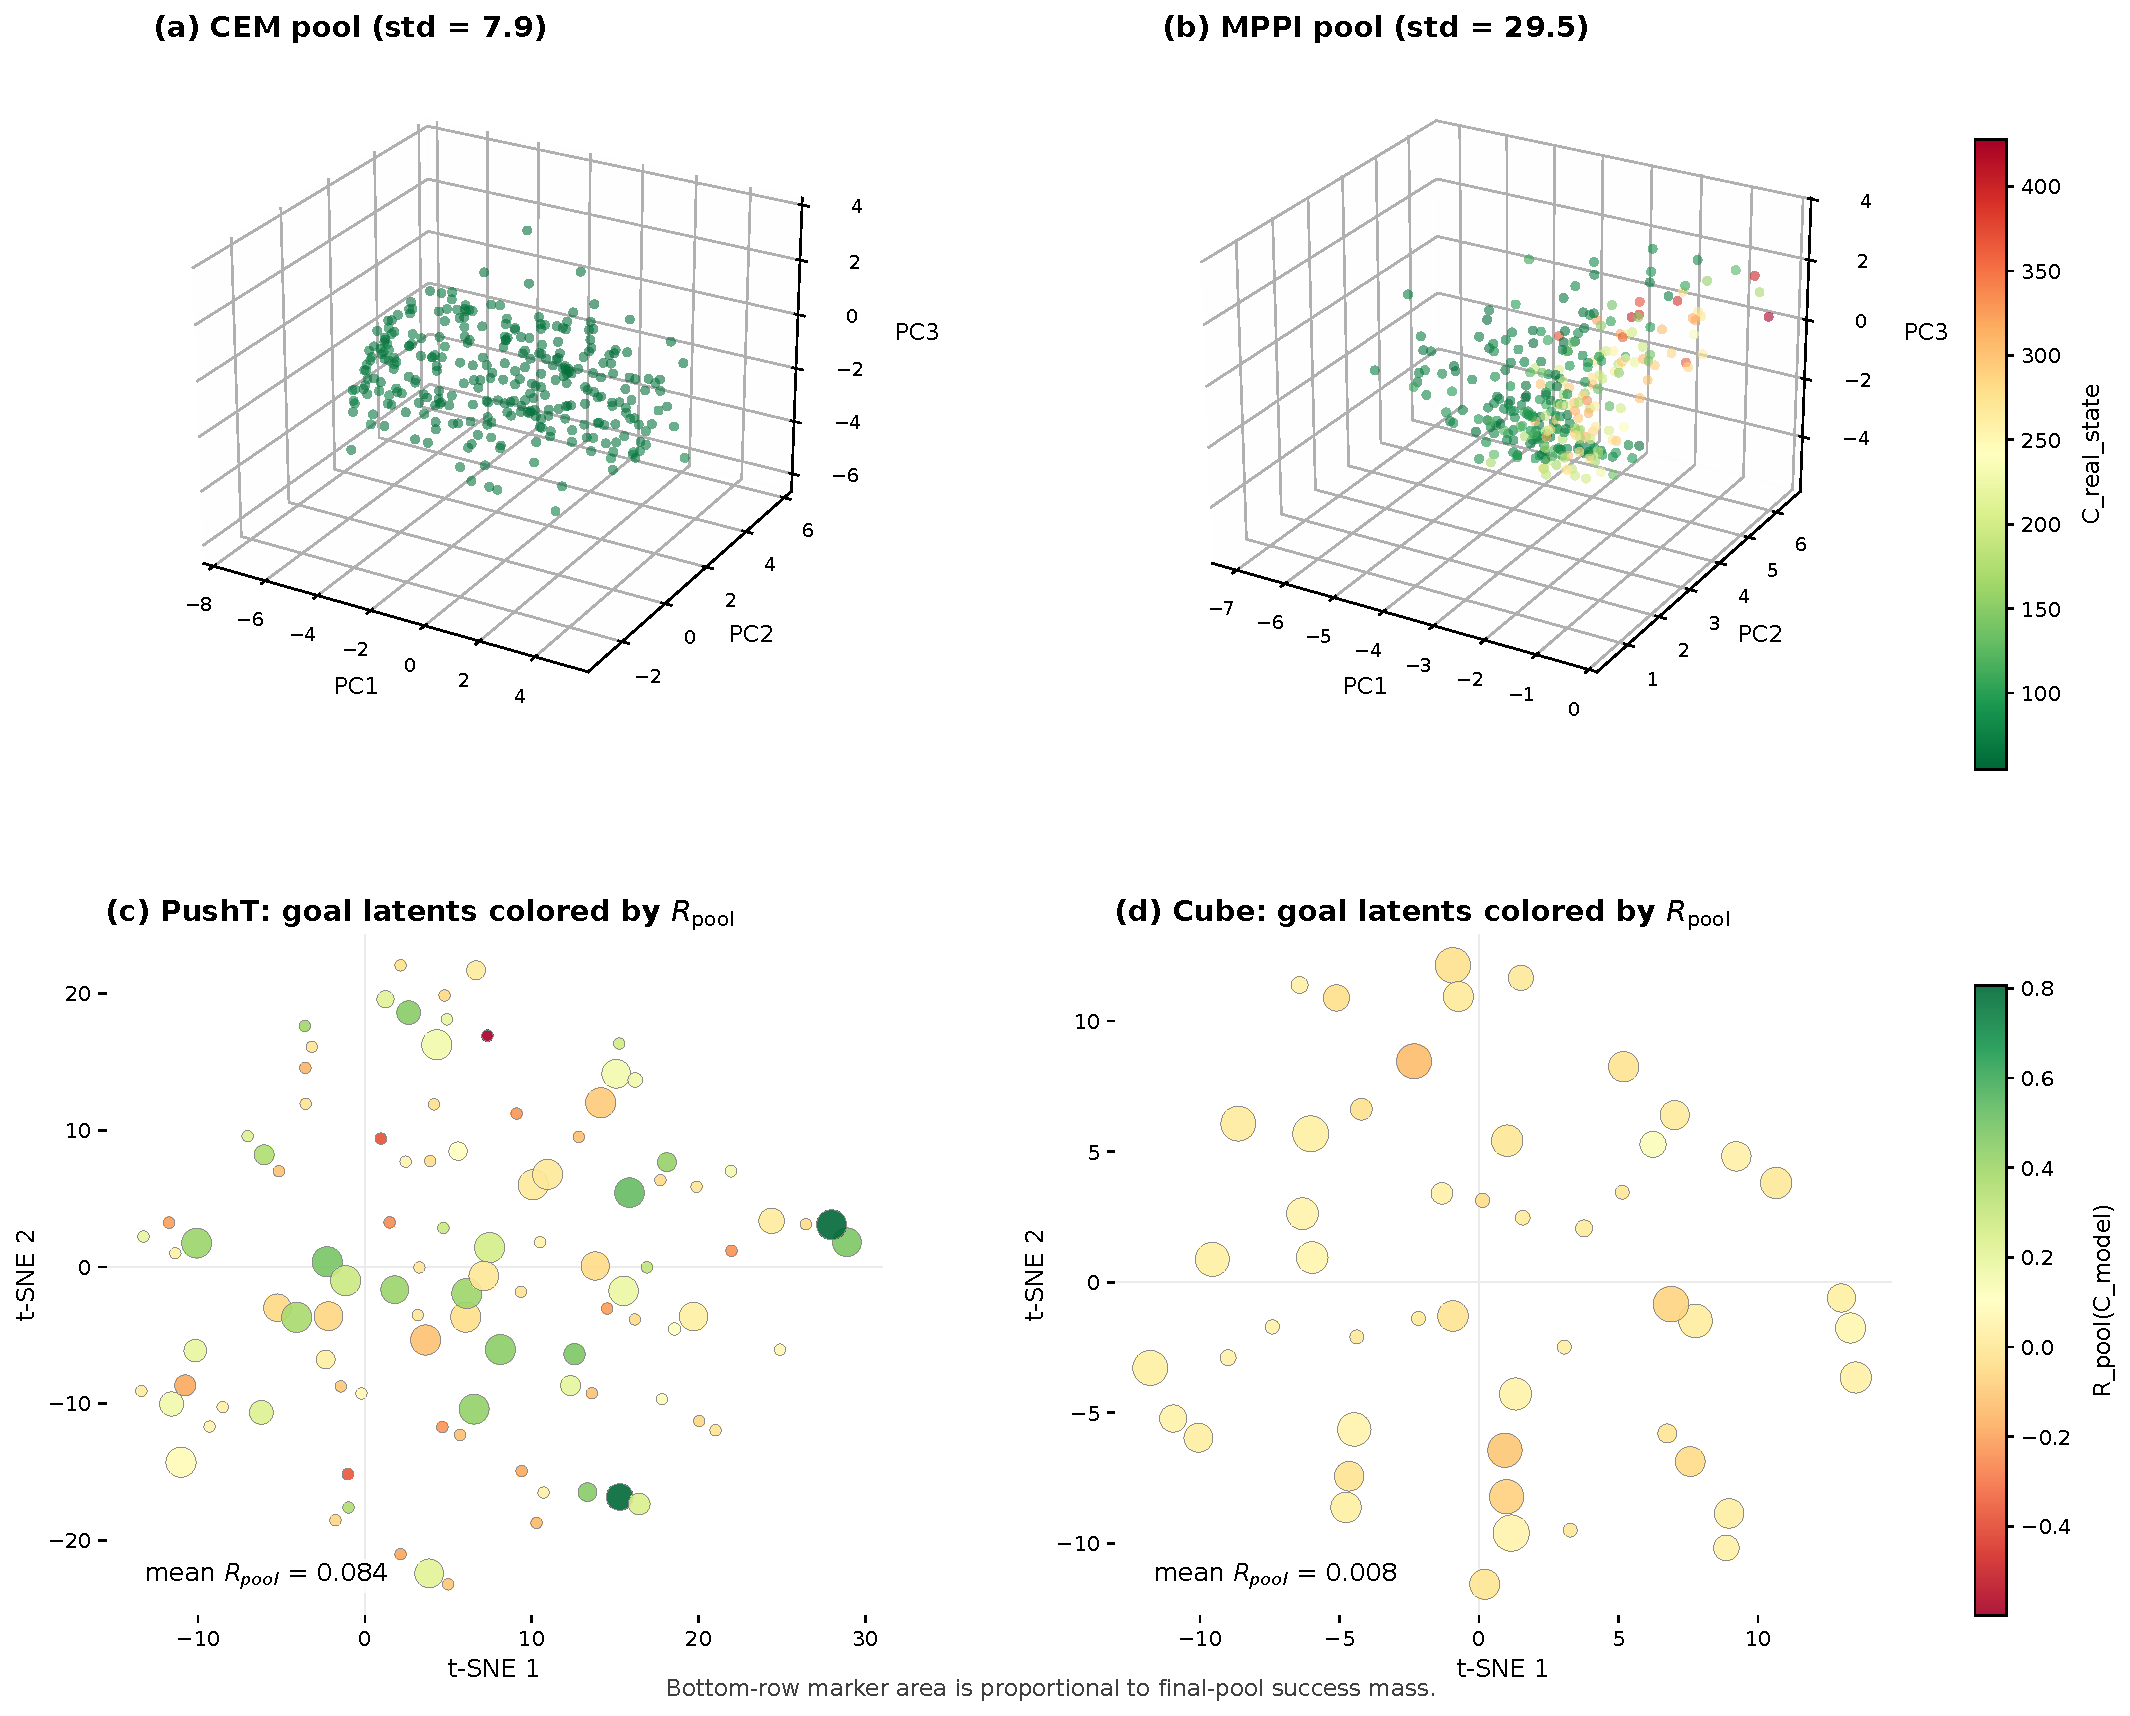
\includegraphics[width=\textwidth]{figures/fig6_spatial.pdf}
\caption{Spatial diagnostics for optimizer and cross-environment analysis. \textbf{(a,b)}~CEM compresses the candidate pool into a tight latent-space cluster ($\mathrm{std}=\mathbf{7.9}$), while MPPI with soft weighting preserves 3.7$\times$ more physical diversity ($\mathrm{std}=\mathbf{29.5}$); both pools are shown for pair~61 under the same PCA projection, colored by physical cost $C_{\text{real\_state}}$. \textbf{(c,d)}~Goal-latent t-SNE maps for PushT (100 pairs) and OGBench-Cube (50 pairs), colored by $\Rpool(\Cmodel)$ with marker area proportional to pool success mass. Near-zero $\Rpool$ (yellow/red) dominates both environments, confirming cross-environment consistency of endpoint-planning decoupling.}
\label{fig:spatial_evidence}
\end{figure*}

The MPPI comparison therefore serves as an optimizer-dependence sanity check rather than a precise attribution of the gap. Soft weighting preserves more physical pool diversity (3.7$\times$) and modestly improves $\Rpool(\Cmodel)$, but it does not close the endpoint-pool gap. Using $\Rendpoint=0.495$ at $m=192$ as the reference, MPPI retains only about 39\% of the endpoint ranking signal ($0.194/0.495$). The wide paired-bootstrap confidence interval for the CEM-specific fraction ($[-16,48]\%$) precludes a precise decomposition. The qualitative finding is that most of the decoupling persists under soft weighting.

\subsection{Cross-Model Validation: DINO-WM}
\label{sec:dinowm}

DINO-WM \citep{zhou2024dinowm} uses a frozen DINOv2 ViT-S/14 encoder with a ViT-style causal Transformer predictor. Its terminal cost combines MSE over predicted visual patch features with proprioceptive MSE, optimized by CEM with the same 300/30/30 configuration as LeWM.

\begin{table}[t]
\centering
\caption{Cross-model comparison of pool-level ranking on PushT. Both models exhibit near-zero $R_{\text{pool}}$ despite different architectures, encoders, and cost functions. DINO-WM results use 29 of the same 30 Track~A pairs (one pair excluded due to scoring timeout).}
\label{tab:cross_model}
\begin{tabular}{lcc}
\toprule
Metric & LeWM & DINO-WM \\
\midrule
Encoder & Learned JEPA & Frozen DINOv2 ViT-S/14 \\
Predictor & Linear/MLP & ViT causal Transformer \\
Terminal cost & $\|z - z_g\|^2$ & MSE patches + $\alpha$ MSE proprio \\
$R_{\text{pool}}(C_{\text{model}})$ & 0.084 & 0.002 \\
Pool $C_{\text{model}}$ std & 2.11 & 0.063 \\
Pool $C_{\text{real}}$ std & 7.84 & 60.6 \\
Planning success & 29.6\% & 3.4\% \\
Selection regret & 19.2 & 128.6 \\
\bottomrule
\end{tabular}
\end{table}

Both models exhibit near-zero pool-level ranking ($R_{\text{pool}} \approx 0$) with severe cost compression (pool $C_{\text{model}}$ standard deviation orders of magnitude below pool $C_{\text{real}}$ standard deviation), confirming that the endpoint-planning decoupling is not specific to LeWM's learned encoder or Euclidean cost. DINO-WM's frozen DINOv2 features and patch-level MSE cost produce the same structural failure: the terminal cost compresses in the CEM-converged region and loses local order preservation. Notably, DINO-WM also shows weak endpoint ranking ($R_{\text{endpoint}} \approx 0.003$), suggesting that the frozen visual encoder may lack task-relevant structure even globally, compounding the local pool-level failure.

These results demonstrate that the three-level diagnostic protocol proposed in this paper applies directly to architecturally distinct latent planners and reveals failure modes that would be invisible under endpoint-only evaluation.

\section{Limitations and Frozen Exclusions}

% REVISION: addresses W1
The evidence has bounded scope. While the primary audit targets LeWM, we validate the core diagnostic on DINO-WM (Section~\ref{sec:dinowm}), confirming cross-model generality on PushT. Cross-environment generalization beyond manipulation tasks remains future work. The environments also do not cover locomotion, navigation, deformable objects, multi-object interaction, semantic planning, broad exploration data, mixed-quality behavior, or online collection.

% REVISION: addresses W3
Cube-specific evidence remains narrower than PushT but is strengthened by the extended full projected-CEM run: the full projected-CEM cell uses the first 50 Cube pairs with three projection seeds, while the Cube re-rank-only cell uses all 100 pairs with three seeds. This supports the cross-environment $\DeltaCEM$ claim, but Cube still has fewer full-planning pairs than PushT and should not be interpreted as a complete environment-general validation.

We report seed-level variance and, for the revised core quantities, bootstrap confidence intervals. These intervals quantify pair-level uncertainty for the main pool-ranking and optimizer-attribution metrics, but the paper still relies primarily on locked decision rules, replicated seeds, and cross-protocol consistency rather than broad hypothesis testing.

% REVISION: addresses W5
The physical task costs used for pool metrics are privileged evaluation signals: appropriate for diagnosis, but unavailable to a deployed planner. The proposed protocol is an evaluation protocol, not a new planning objective. Our privilege-free proxy analysis suggests that learned-cost spread can partially monitor high-regret cases without simulator access, but this proxy has only been validated on PushT and does not yet replace $\Rpool$ or selection-regret measurement across environments.

% REVISION: addresses W4
CEM remains the primary optimizer studied in this paper. The MPPI comparison on a 30-pair PushT subset (90 scored pools across three seeds) provides partial cross-optimizer evidence: soft weighting preserves more physical pool diversity and improves $\Rpool(\Cmodel)$, but it does not close the endpoint-pool gap. Gradient-based planners, learned proposals, value-guided search, and closed-loop replanning may interact differently with the same latent geometry and would require their own optimizer-local pool definitions.

Subspace-CEM was tested at smoke scale: 30 pairs, two seeds, $m=64$. A wider search over projection dimensions, iteration schedules, or re-ranking pool sizes could differ; we stopped because the pre-registered criterion was not met.

Frozen exclusions include multi-step rollout training, closed-loop SIGReg, drift-aware CEM, and hierarchical world modeling; they define scope, not permanent claims.


\bibliographystyle{iclr2025_conference}
\bibliography{references}

\newpage
\appendix

\section{Reproducibility and Setup}
\label{app:reproducibility}

\subsection{Hardware}

All results use fixed public LeWM checkpoints and no additional LeWM training. Local
development and most PushT analyses were run on the Apple Silicon workstation
recorded in the repository setup notes: macOS 26.3 ARM on an Apple M5 Pro, using
PyTorch MPS when available. The MPS device is visible from a normal host
terminal; the Codex sandbox can fail to expose Metal devices, so all MPS claims
refer to host-terminal runs. The RunPod closeout record reports an NVIDIA RTX
5090 server with CUDA 13.0 and 32GB VRAM for the final GPU-only checks. The
repository also includes \texttt{scripts/setup\_runpod.sh}, whose header targets
a fresh RunPod instance with system Python 3.12, CUDA 12.8, and pre-installed
\texttt{torch}/\texttt{torchvision}; the closeout log is the source for the
actual final RunPod runtime.

\begin{table}[h]
\centering
\scriptsize
\begin{tabular}{p{0.22\linewidth}p{0.28\linewidth}p{0.40\linewidth}}
\toprule
Hardware & Evidence in repo & Experiments run there \\
\midrule
Apple Silicon MPS workstation & \texttt{README.md}; \texttt{progress\_log.md}; \texttt{mps\_setup.md} & Phase 0 PushT/Cube baselines and sweeps; Track A 100-pair PushT artifact and three-cost pass; Stage 1A controls; Stage 1B PushT full projected CEM; PushT re-rank-only protocol matching; Cube Stage 1B re-rank-only; P2-0 learned-cost, DINOv2, and hybrid-CEM analyses. \\
RunPod RTX 5090 GPU server & \texttt{closeout\_session\_summary.md} & Cube anomaly multi-seed sanity; PushT Subspace-CEM Stage A; CUDA-side Cube full projected CEM/protocol matching artifacts. \\
CPU / offline aggregation & Artifact metadata and memos & Orthogonal sanity check, CEM-gap aggregation, taxonomy table, paper figure generation, and LaTeX compilation. \\
\bottomrule
\end{tabular}
\caption{Compute placement for the main audit artifacts.}
\label{tab:appendix-hardware}
\end{table}

\subsection{Software Environment}

The standard local setup command is \texttt{bash scripts/setup\_env.sh}. This
creates the \texttt{lewm-audit} conda environment with Python 3.11. The requested
search for environment YAML files returned no \texttt{*.yml} or \texttt{*.yaml}
environment file, so the repository should be treated as script-configured rather
than YAML-configured. The setup and progress logs verify
\texttt{stable-worldmodel==0.0.6}, editable
\texttt{stable-pretraining==0.1.7.dev44+gd8d8f568d.d20260501},
\texttt{ogbench==1.2.1}, and local PyTorch
\texttt{2.13.0.dev20260430}. RunPod final checks used miniconda,
\texttt{lewm-audit}, and PyTorch \texttt{2.11+cu128} according to the closeout
summary; the one-shot RunPod script installs \texttt{stable-worldmodel[train]},
\texttt{ogbench}, \texttt{gymnasium}, \texttt{opencv-python-headless},
\texttt{matplotlib}, \texttt{seaborn}, \texttt{scipy}, and
\texttt{scikit-learn} after confirming the pre-installed PyTorch package.

The only tracked local patch is \texttt{patches/lewm\_mps\_fix.patch}. It changes
the upstream LeWM \texttt{jepa.py} tensor-transfer path so that floating tensors
moved to an MPS device are cast to \texttt{torch.float32}; without this safeguard, MPS
rejects upstream \texttt{float64} tensors. Re-application instructions are in
\texttt{docs/mps\_setup.md}. The paper was compiled with \texttt{tectonic
main.tex} from \texttt{paper/}, using the ICLR 2025 template.

\begin{table}[h]
\centering
\scriptsize
\begin{tabular}{p{0.24\linewidth}p{0.32\linewidth}p{0.34\linewidth}}
\toprule
Component & Recorded version or setting & Source \\
\midrule
Conda environment & \texttt{lewm-audit} & \texttt{README.md}; setup scripts \\
Python & \texttt{3.11} local; system Python 3.12 targeted by RunPod script & \texttt{README.md}; setup scripts \\
\texttt{stable-worldmodel} & \texttt{0.0.6} local verified install & \texttt{README.md}; progress log \\
\texttt{stable-pretraining} & \begin{tabular}[t]{@{}l@{}}\texttt{0.1.7.dev44+}\\\texttt{gd8d8f568d.d20260501}\end{tabular} editable install & \texttt{README.md}; progress log \\
\texttt{ogbench} & \texttt{1.2.1} local verified install & \texttt{README.md}; progress log \\
PyTorch & \texttt{2.13.0.dev20260430} local MPS; \texttt{2.11+cu128} RunPod closeout & \texttt{README.md}; closeout summary \\
CUDA / GPU & CUDA 13.0, RTX 5090, 32GB VRAM for final RunPod runs & closeout summary \\
LaTeX & \texttt{tectonic main.tex} & closeout summary \\
\bottomrule
\end{tabular}
\caption{Software versions recorded in setup scripts and progress logs.}
\label{tab:appendix-software}
\end{table}

\subsection{Checkpoints}

Checkpoint download is handled by \texttt{scripts/download\_checkpoints.sh} on
local machines and by the equivalent checkpoint step in
\texttt{scripts/setup\_runpod.sh} on RunPod. Both scripts use the Hugging Face
CLI, with repository type \texttt{model}, to download the official public LeWM
checkpoint repositories. The root README links the LeWM Hugging Face collection
at \url{https://huggingface.co/collections/quentinll/lewm}. The exact Hugging
Face snapshot revision was not pinned at the time of the audit. All numerical
results are reproducible from the frozen JSON artifacts listed in
Table~\ref{tab:appendix-commits}.

\begin{table}[h]
\centering
\scriptsize
\setlength{\tabcolsep}{3pt}
\begin{tabular}{p{0.15\linewidth}p{0.21\linewidth}p{0.27\linewidth}p{0.25\linewidth}}
\toprule
Environment & Hugging Face model ID & Raw local files & Converted checkpoint \\
\midrule
PushT & \texttt{quentinll/lewm-pusht} & \begin{tabular}[t]{@{}l@{}}\texttt{weights.pt} and\\\texttt{config.json} under\\\texttt{checkpoints/lewm-pusht/}\end{tabular} & \begin{tabular}[t]{@{}l@{}}\texttt{lewm\_object.ckpt}\\under \texttt{checkpoints/}\\\texttt{converted/lewm-pusht/}\end{tabular} \\
OGBench-Cube & \texttt{quentinll/lewm-cube} & \begin{tabular}[t]{@{}l@{}}\texttt{weights.pt} and\\\texttt{config.json} under\\\texttt{checkpoints/lewm-cube/}\end{tabular} & \begin{tabular}[t]{@{}l@{}}\texttt{lewm\_object.ckpt}\\under \texttt{checkpoints/}\\\texttt{converted/lewm-cube/}\end{tabular} \\
\bottomrule
\end{tabular}
\caption{Official public LeWM checkpoints used by the audit.}
\label{tab:appendix-checkpoints}
\end{table}

\texttt{scripts/verify\_checkpoint.py} reconstructs the LeWM \texttt{JEPA} model
from \texttt{config.json}, loads \texttt{weights.pt}, saves a
\texttt{stable\_worldmodel.policy.AutoCostModel}-compatible object checkpoint as
\texttt{lewm\_object.ckpt}, and verifies load plus forward passes. The progress
log records that both PushT and Cube checkpoint files are about 69MB, that the
converted checkpoints produce encoder embeddings of shape \((1,192)\), and that
predictor verification produced shape \((1,3,192)\). The verified model has
about 18.0M parameters: 5.5M in the encoder and 12.5M in the predictor stack.
PushT uses raw action dimension 2 and effective checkpoint action dimension 10;
Cube uses raw action dimension 5 and effective checkpoint action dimension 25,
matching \texttt{action\_block=5}.

\subsection{Evaluation Seeds}

The audit uses fixed dataset-pair artifacts where possible and then varies only
the intended stochastic object. For Phase 0 baselines and offset sweeps, the
default command-line seed is 42. The later paper artifacts use seed 0 for fixed
pair selection, CEM sampling base seeds, and single-run controls unless a
multi-seed check is explicitly listed. Gaussian projection matrices have shape
\([192,m]\), entries \(\mathcal{N}(0,1)/\sqrt{m}\), and are fixed per
\((m,\texttt{projection\_seed})\) across pairs and CEM iterations.

\begin{table}[h]
\centering
\small
\begin{tabular}{p{0.28\linewidth}p{0.28\linewidth}p{0.34\linewidth}}
\toprule
Artifact or phase & Seeds & Notes \\
\midrule
Phase 0 PushT/Cube baselines and offset sweeps & 42 & Defaults in \texttt{eval\_pusht\_baseline.py}, \texttt{eval\_pusht\_sweep.py}, \texttt{eval\_cube\_baseline.py}, and \texttt{eval\_cube\_sweep.py}. \\
Track A PushT pair set and three-cost artifact & 0 & \texttt{track\_a\_pairs.json} and \texttt{track\_a\_three\_cost.json}; 100 pairs, 80 actions per pair. \\
Stage 1A C1-C5 controls & 0--9 & Ten-seed orthogonal, Gaussian projection, coordinate subset, Gaussian null, and shuffle controls. \\
Stage 1A C0/C6/C7 & 0 or deterministic single run & C0 is trained LeWM; C6 is randomly initialized LeWM seed 0; C7 DINOv2 feature extraction records seed 0. \\
Stage 1B PushT full projected CEM & base seed 0; projection seeds 0,1,2 & 63-pair smoke/full record; later full artifact uses dimensions 1--192 and the same projection seed set. \\
PushT re-rank-only protocol matching & base seed 0; projection seeds 0,1,2 & 100 pairs, 9 projection dimensions, 2700 projected records. \\
Cube Stage 1B re-rank-only & base seed 0; projection seeds 0,1,2 & 100 Cube pairs, 9 projection dimensions, 2700 projected records. \\
Cube full projected CEM smoke & base seed 0; projection seed 0 & 25 selected Cube pairs, dimensions \(\{1,8,32,64,192\}\). \\
Cube anomaly sanity & projection seeds 0,1,2 & Seed 0 from \texttt{cube\_full\_proj\_cem.json}; added seeds 1 and 2 in \texttt{cube\_anomaly\_sanity.json}. \\
P2-0 learned costs and hybrid CEM & 0 & Cost-head splits, planning evaluation, and oracle-budget sweeps record seed 0. \\
PushT Subspace-CEM Stage A & 0,1 & 30 pairs, \texttt{m=64} search with full-dimensional re-rank. \\
\bottomrule
\end{tabular}
\caption{Seed policy by experimental phase.}
\label{tab:appendix-seeds}
\end{table}

\subsection{Statistical Uncertainty}

Table~\ref{tab:appendix-uncertainty} collects the uncertainty intervals added
for the second-round revision.  The bootstrap intervals use the pair or
paired-pair experimental unit rather than individual candidates, and binary
repair outcomes use exact binomial intervals.

% Generated by scripts/revision/appendix_uncertainty_table.py
\begin{table*}[p]
\centering
\scriptsize
\setlength{\tabcolsep}{2.5pt}
\resizebox{\textwidth}{!}{%
\begin{tabular}{@{}L{0.18\textwidth}L{0.07\textwidth}L{0.20\textwidth}L{0.05\textwidth}L{0.06\textwidth}L{0.15\textwidth}L{0.12\textwidth}L{0.15\textwidth}@{}}
\toprule
Metric & Env. & Protocol / experiment & $N$ & Seeds & Point estimate & 95\% CI & Method \\
\midrule
$R_\mathrm{endpoint}$ ($m=64$) & PushT & Stage 1A C2 endpoint projection & 100 & 10 proj. & 0.473 & [0.395, 0.543] & pair bootstrap \\
$R_\mathrm{endpoint}$ ($m=192$) & PushT & Stage 1A C2 endpoint projection & 100 & 10 proj. & 0.495 & [0.411, 0.570] & pair bootstrap \\
$R_\mathrm{pool}(C_\mathrm{model})$ & PushT & Default CEM final pools & 100 & 1 & 0.084 & [0.037, 0.131] & pair bootstrap \\
$R_\mathrm{pool}(C_\mathrm{V3})$ & PushT & Actual-terminal encoder ranker & 100 & 1 & 0.258 & [0.146, 0.365] & pair bootstrap \\
$R_\mathrm{pool}(C_\mathrm{V1})$ & PushT & Physical hinge ranker & 100 & 1 & 0.666 & [0.595, 0.735] & pair bootstrap \\
$\Delta_\mathrm{CEM}$ & PushT & C0 endpoint ref. minus default pool & 100 & 1 & 0.422 & [0.374, 0.468] & pair bootstrap \\
$R_\mathrm{pool}(C_\mathrm{model})$ & Cube & Full projected CEM, $m=64$ & 50 & 3 proj. & -0.001 & [-0.018, 0.016] & pair bootstrap \\
$\Delta_\mathrm{CEM}$ & Cube & Endpoint $m=64$ minus full CEM pool & 50 & 3 proj. & 0.576 & [0.559, 0.594] & pair bootstrap \\
\addlinespace
$R_\mathrm{pool}(C_\mathrm{model})$ diff. & PushT & MPPI minus CEM & 30 & 3 & 0.079 (0.115 to 0.194) & [-0.044, 0.204] & paired bootstrap \\
Planning success diff. & PushT & MPPI minus CEM & 30 & 3 & -14.4 pp (53.3\% to 38.9\%) & [-26.7, -2.2] pp & paired bootstrap \\
Pool $C_\mathrm{real}$ std diff. & PushT & MPPI minus CEM & 30 & 3 & 21.530 (7.947 to 29.478) & [17.151, 25.854] & paired bootstrap \\
MPPI attribution fraction & PushT & CEM-to-MPPI gap fraction & 30 & 3 & 22.225\% & [-15.736, 48.094]\% & paired bootstrap \\
\addlinespace
Cost head Split 3 success & PushT & Learned cost repair & 16 & 1 & 0/16 (0.000\%) & [0.000, 20.591]\% & Clopper-Pearson \\
Cost head CEM-aware success & PushT & Learned cost repair & 16 & 1 & 1/16 (6.250\%) & [0.158, 30.232]\% & Clopper-Pearson \\
DINOv2 gap vs. LeWM & PushT & Track B endpoint replacement & 100 & 1 & 0.242 (0.261 vs. 0.503) & [0.115, 0.368] & pair bootstrap \\
Subspace-CEM success delta & PushT & Subspace minus default CEM & 30 & 2 & -8.3 pp (56.7\% to 48.3\%) & [-18.3, 0.0] pp & paired bootstrap \\
Hybrid CEM 20\% threshold & PushT & V1 oracle re-rank, $K=60$ & 16 & 1 & 7/16 (43.750\%) & [19.753, 70.122]\% & Clopper-Pearson \\
\bottomrule
\end{tabular}%
}
\caption{Uncertainty summary for the main endpoint-pool, optimizer, and repair metrics. Bootstrap intervals use 10{,}000 resamples over the experimental unit shown in the Method column. Exact intervals are Clopper--Pearson binomial intervals. Endpoint global Spearman intervals bootstrap pair clusters after rank-transforming endpoint records, so the point estimates match the global Spearman values reported in the main tables.}
\label{tab:appendix-uncertainty}
\end{table*}


\subsection{Reproducibility Notes}

The main fixed artifacts record the commit that generated them. The repository
history has continued after these pre-registration and closeout points, so the
artifact-level commit hashes are the reproducibility anchors rather than the
current branch head alone.

\begin{table}[h]
\centering
\scriptsize
\begin{tabular}{p{0.30\linewidth}p{0.22\linewidth}p{0.38\linewidth}}
\toprule
Anchor & Commit & Evidence \\
\midrule
Track A stratified pair artifact & \texttt{3ac6afa93c98} & \texttt{track\_a\_pairs.json} \\
Track A three-cost pass & \texttt{45d65afc1546} & \texttt{track\_a\_three\_cost.json} \\
Stage 1B smoke / full projected CEM & \texttt{7848d5b00f28}, \texttt{a48f9f3d0e18} & \texttt{stage1b\_smoke\_memo.md}; \texttt{stage1b\_full.json} \\
PushT re-rank-only and Cube Stage 1B & \texttt{a3388de9d6dc} & \texttt{pusht\_rerank\_only.json}; \texttt{cube\_stage1b.json} \\
Cube full projected CEM & \texttt{485b3390154f} & \texttt{cube\_full\_proj\_cem.json} \\
Protocol-matching memo & \texttt{7917feb3996e} & \texttt{protocol\_matching\_memo.md} \\
PushT Subspace-CEM Stage A & \texttt{adc573ac8c2b} & \texttt{stage\_a\_pusht.json} \\
\bottomrule
\end{tabular}
\caption{Commit anchors recorded by the reproducibility artifacts.}
\label{tab:appendix-commits}
\end{table}

Known non-determinism comes from stochastic CEM sampling, simulator rollouts,
random projections, GPU kernels, and backend differences between MPS and CUDA.
The code sets Python, NumPy, and PyTorch seeds in the Phase 2 evaluators where
the scripts expose a seed; CUDA scripts call \texttt{torch.cuda.manual\_seed\_all}
when CUDA is available. Some finite-sample baseline variation is expected: for
example, the reproduced PushT baseline is 98\% on 50 episodes versus the paper
reference point of 96\%, and Cube baseline is 66\% on 50 episodes versus the
paper reference point of 74\%.

Runtime estimates recorded in the repository are as follows. PushT MPS baseline
evaluation takes about 295 seconds for 50 episodes, with a one-time first-solve
shader warmup. The PushT offset sweep took about 1 hour on MPS. The Track A
100-pair three-cost run took about 9 minutes from its recorded start and finish
timestamps. PushT re-rank-only and Cube full projected CEM each report about
5 minutes 16 seconds. Cube Stage 1B re-rank-only reports about 1 hour 19
minutes. Final RunPod closeout runs report 7 minutes 8 seconds for the Cube
anomaly sanity check and 4 minutes 23 seconds for PushT Subspace-CEM Stage A.

\section{Phase 0 Full Results}
\label{app:phase0}

Phase~0 reproduced the LeWM baselines on both environments and ran offset
sweeps, three-cost attribution, per-pair categorization, and aggregate latent
diagnostics.  These results motivated the audit framing developed in
Sections~3--4 of the main text.

\subsection{PushT Baseline and Offset Sweep}

The PushT baseline was reproduced at 98\% success on 50 episodes (paper
reference: 96\%; the difference is within finite-sample variation at $n=50$).
Table~\ref{tab:pusht-offset} reports the offset sweep.  Planning success drops
sharply beyond offset~25, falling from 96\% to 10\% at offset~100.  All runs
used seed~42 on Apple Silicon MPS; the full sweep took approximately one hour.
These numbers are plotted in Figure~\ref{fig:motivation}a.

\begin{table}[h]
\centering
\caption{PushT planning success versus goal offset.  Each row evaluates 50
episodes at the indicated offset (number of environment steps between the
initial observation and the goal observation in the expert demonstration).}
\label{tab:pusht-offset}
\begin{tabular}{lcccc}
\toprule
Goal offset (steps) & 25 & 50 & 75 & 100 \\
\midrule
Success rate (\%) & 96 & 58 & 16 & 10 \\
Successes / episodes & 48/50 & 29/50 & 8/50 & 5/50 \\
\bottomrule
\end{tabular}
\end{table}

\subsection{Cube Baseline and Offset Sweep}

The OGBench-Cube baseline was reproduced at 66\% on 50 episodes (paper
reference: 74\%).  Unlike PushT, Cube success does not degrade with goal
offset: it remains between 50\% and 68\% across all four offsets
(Table~\ref{tab:cube-offset}).  This flat curve indicates a
horizon-independent visual encoding difficulty rather than the
displacement-dependent breakdown observed in PushT.  Cube entered the audit
at Phase~2 with its own 100-pair stratified artifact (Appendix~\ref{app:stage1b}).

\begin{table}[h]
\centering
\caption{OGBench-Cube planning success versus goal offset.  Each row evaluates
50 episodes.  Success is defined by
$\|x_\text{cube}^\text{terminal} - x_\text{cube}^\text{goal}\|_2 \le 0.04$.}
\label{tab:cube-offset}
\begin{tabular}{lcccc}
\toprule
Goal offset (steps) & 25 & 50 & 75 & 100 \\
\midrule
Success rate (\%) & 68 & 50 & 58 & 50 \\
Successes / episodes & 34/50 & 25/50 & 29/50 & 25/50 \\
\bottomrule
\end{tabular}
\end{table}

\subsection{Three-Cost Attribution}
\label{app:three-cost}

At offset~50, 30 PushT diagnostic pairs were each evaluated with 40 candidate
actions (10 per source: expert data, random, CEM-early, CEM-late; 1{,}200
records total).  Three pairwise Spearman correlations decompose the end-to-end
cost alignment into a predictor-fidelity term and an encoder-physics term:

\begin{itemize}
\item \textbf{Predictor fidelity} $\rho(\Cmodel,\, C_\text{real\_z})$: how
  well the imagined terminal latent from the predictor tracks the real
  terminal latent.
\item \textbf{Encoder-physics alignment}
  $\rho(C_\text{real\_z},\, C_\text{real\_state})$: how well latent distance
  from the \emph{real} terminal encoding tracks physical task cost.
\item \textbf{End-to-end alignment}
  $\rho(\Cmodel,\, C_\text{real\_state})$: the product-path correlation that
  CEM planning ultimately depends on.
\end{itemize}

\noindent
Here $\Cmodel = \|\zhatH - \zgoal\|^2$ is the model cost used by CEM,
$C_\text{real\_z} = \|z_\text{terminal} - \zgoal\|^2$ uses the encoder
applied to the actual terminal observation, and
$C_\text{real\_state}$ is the V1 hinge cost combining block position error
and angle error.

Table~\ref{tab:three-cost} reports both global (all 1{,}200 records pooled)
and per-pair (mean $\pm$ SEM over 30 pairs) correlations.  Predictor fidelity
is high in both views.  Encoder-physics alignment is moderate globally but
weak and heterogeneous per pair: 6 of 30 pairs have negative
$\rho(C_\text{real\_z}, C_\text{real\_state})$, and the per-pair standard
deviation is 0.502.  This heterogeneity motivates the per-subset analysis in
Appendix~\ref{app:track_a} and the endpoint-planning decoupling framework in
Section~4.  These per-pair means are plotted in Figure~\ref{fig:motivation}b.

\begin{table}[h]
\centering
\caption{Three-cost attribution at PushT offset~50.  Global correlations pool
all 1{,}200 records; per-pair correlations average 30 within-pair Spearman
values ($\pm$\,SEM).}
\label{tab:three-cost}
\begin{tabular}{lcc}
\toprule
Correlation pair & Global Spearman & Per-pair Spearman (mean $\pm$ SEM) \\
\midrule
Predictor fidelity: $\rho(\Cmodel, C_\text{real\_z})$ & 0.864 & 0.779 $\pm$ 0.030 \\
Encoder-physics: $\rho(C_\text{real\_z}, C_\text{real\_state})$ & 0.669 & 0.353 $\pm$ 0.092 \\
End-to-end: $\rho(\Cmodel, C_\text{real\_state})$ & 0.596 & 0.332 $\pm$ 0.085 \\
\bottomrule
\end{tabular}
\end{table}

\subsection{Per-Pair Categorization}
\label{app:per-pair-cat}

The 30 offset-50 pairs were categorized by the number of successful actions
among their 40 candidates (Table~\ref{tab:pair-categories}).  This
categorization informed Phase~1 Track~A stratified sampling
(Appendix~\ref{app:track_a}): the 100-pair artifact was designed to cover the
full displacement$\times$rotation grid, including cells where Phase~0 found
zero-success pairs.

\begin{table}[h]
\centering
\caption{Per-pair categorization at PushT offset~50 ($n=30$ pairs, 40 actions
each).  Block displacement is the Euclidean distance between initial and goal
block positions in pixel coordinates.}
\label{tab:pair-categories}
\begin{tabular}{lccccc}
\toprule
Category & Definition & Count & Mean success & Mean displacement & Mean latent dist.\ \\
\midrule
Easy & $>$25/40 successes & 8 & 80.9\% & 2.57 & 12.50 \\
Hard & 1--25/40 successes & 15 & 21.2\% & 66.01 & 18.84 \\
Impossible & 0/40 successes & 7 & 0.0\% & 123.27 & 19.36 \\
\bottomrule
\end{tabular}
\end{table}

The ``Impossible'' pairs have zero successful actions in the 40-candidate pool,
indicating that the CEM search space does not contain solutions at these
displacements.  Their mean block displacement (123.3 pixels) is roughly 48$\times$
larger than the Easy pairs (2.6 pixels), while their mean latent distance
(19.4) is only 1.55$\times$ larger, illustrating the compression of physical
task structure in the learned latent geometry.

\subsection{Aggregate Latent Diagnostics}
\label{app:latent-diag}

Phase~0 also evaluated aggregate properties of the LeWM latent space over 100
randomly sampled trajectories (10 latent steps each, action blocks of 5;
seed~42).  Table~\ref{tab:latent-diagnostics} compares real encoder latents
with predictor-imagined latents.

\begin{table}[h]
\centering
\caption{Aggregate latent diagnostics for LeWM PushT.  Real latents use the
encoder applied to ground-truth observations; imagined latents use the
predictor rolled forward from the initial observation.  Effective rank is the
exponentiated entropy of the normalized singular-value spectrum.
Participation rank is $(\text{tr}\,\Sigma)^2 / \|\Sigma\|_F^2$.}
\label{tab:latent-diagnostics}
\begin{tabular}{lcc}
\toprule
Metric & Real latents & Imagined latents \\
\midrule
Temporal straightness (mean $\pm$ std) & 0.516 $\pm$ 0.301 & 0.531 $\pm$ 0.299 \\
Effective rank & 107.3 & 106.1 \\
Participation rank & 63.9 & 63.1 \\
Top-1 variance fraction & 3.40\% & 3.50\% \\
Top-10 variance fraction & 25.9\% & 26.2\% \\
Covariance trace & 190.0 & 190.0 \\
\bottomrule
\end{tabular}
\end{table}

Prediction error grows with rollout horizon: mean $\ell_2$ distance between
real and imagined latents rises from 1.10 at step~1 to 5.83 at step~10
(Table~\ref{tab:pred-error}).  Despite this drift, imagined latents preserve
aggregate distributional properties: effective rank, participation rank, and
covariance spectrum are nearly identical between real and imagined latents.
This confirms that the predictor does not collapse the representation, and the
planning failure is not attributable to predictor divergence in aggregate.

\begin{table}[h]
\centering
\caption{Predictor rollout error by horizon step.  $\ell_2$ distance is
computed between the real encoder latent and the predictor-imagined latent at
each step, averaged over 100 trajectories.}
\label{tab:pred-error}
\begin{tabular}{lcccccccccc}
\toprule
Step & 1 & 2 & 3 & 4 & 5 & 6 & 7 & 8 & 9 & 10 \\
\midrule
Mean $\ell_2$ & 1.10 & 1.59 & 2.17 & 2.50 & 2.87 & 3.40 & 4.00 & 4.52 & 5.14 & 5.83 \\
MSE & .008 & .018 & .048 & .058 & .072 & .101 & .136 & .168 & .215 & .271 \\
\bottomrule
\end{tabular}
\end{table}

The Phase~0 conclusion was that encoder goal geometry, not predictor drift or
planner weakness, is the primary source of long-horizon failure in PushT.  The
predictor faithfully preserves the cost landscape of the encoder, so the CEM
planner optimizes a faithful but misaligned objective.  This conclusion was
later refined by the Track~A analysis (Appendix~\ref{app:track_a}) and the
endpoint-planning decoupling framework (Section~4), which showed that the
misalignment is not a global encoder property but a local interaction between
cost geometry and CEM search dynamics.

\section{Track A Stratified Sampling and Analysis}
\label{app:track_a}

Phase~1 converted the Phase~0 30-pair PushT diagnosis into a 100-pair
stratified artifact at offset~50, with 80 candidate actions per pair split
evenly across four sources (20~data, 20~smooth-random, 20~CEM-early,
20~CEM-late; 8{,}000 records total).  This appendix documents the sampling
grid, failure-mode decomposition, sign-reversal cluster, and D-row cost
diagnosis that underlie the main-text audit trajectory (Section~3.2).

\subsection{Stratified Sampling Grid}
\label{app:track_a_grid}

Pairs were sampled over a $4\times 4$ displacement$\times$rotation grid with
edges $D \in \{0, 10, 50, 120, \infty\}$~pixels and
$R \in \{0, 0.25, 0.75, 1.25, \infty\}$~radians.  Table~\ref{tab:track-a-grid}
reports the per-cell pair count, success rate, and per-pair encoder-physics
Spearman correlation.

\begin{table}[h]
\centering
\caption{Track~A per-cell summary ($4\times 4$ displacement$\times$rotation
grid, 100 pairs, 80 actions each).  Success rate is the fraction of actions
that satisfy the PushT success criterion.  Mean~$\rho$ is the within-pair
Spearman correlation between $C_\text{real\_z}$ and $C_\text{real\_state}$,
averaged over pairs in the cell.}
\label{tab:track-a-grid}
\begin{tabular}{lcccc}
\toprule
 & R0 ($<$0.25) & R1 (0.25--0.75) & R2 (0.75--1.25) & R3 ($>$1.25) \\
\midrule
D0 ($<$10\,px) & 6 / 76.7\% / 0.39 & 6 / 44.6\% / 0.41 & 6 / 32.1\% / 0.32 & 6 / 4.6\% / $-$0.27 \\
D1 (10--50\,px) & 6 / 27.1\% / 0.50 & 6 / 7.5\% / 0.34 & 6 / 19.0\% / 0.14 & 6 / 0.0\% / $-$0.29 \\
D2 (50--120\,px) & 6 / 15.0\% / 0.32 & 6 / 17.3\% / 0.60 & 7 / 0.9\% / 0.08 & 7 / 0.2\% / 0.38 \\
D3 ($>$120\,px) & 6 / 7.9\% / 0.67 & 7 / 11.4\% / 0.73 & 6 / 2.7\% / 0.58 & 7 / 1.8\% / 0.40 \\
\bottomrule
\end{tabular}
\end{table}

No cell was empty; all 16 cells have 6--7 pairs.  Success rate decreases with
both displacement and rotation, but encoder-physics alignment does
\emph{not} follow a simple monotone pattern: D3 cells have higher mean~$\rho$
than D0 cells (see Section~\ref{app:drow} below).

\subsection{DP1 Aggregate Statistics}
\label{app:dp1}

The DP1 diagnostic checks whether per-pair Spearman heterogeneity is
comparable to Phase~0.  Over all 100 pairs, the per-pair Spearman
$\rho(C_\text{real\_z}, C_\text{real\_state})$ has mean 0.333, std 0.477,
and median 0.414 (range $-0.766$ to $+0.914$).  The bootstrapped 95\% CI for
the standard deviation is $[0.412, 0.529]$, above the 0.300 pre-registered
threshold.  Phase~0 reference values (mean 0.353, std 0.486) are within this
interval, confirming that the stratified artifact preserves the heterogeneity
observed in Phase~0.

\subsection{Failure-Mode Decomposition}
\label{app:failure_decomp}

Each of the 100 pairs was classified along two axes: (i)~\emph{success
class}---``all\_fail'' if 0/80 actions succeed, ``some\_succ'' otherwise; and
(ii)~\emph{encoder class}---``neg\_rho'' if per-pair
$\rho(C_\text{real\_z}, C_\text{real\_state}) < 0$, ``weak\_rho'' if
$0 \le \rho < 0.3$, ``strong\_rho'' if $\rho \ge 0.3$.
Table~\ref{tab:failure-decomp} reports the resulting $2\times 3$ count
matrix.

\begin{table}[h]
\centering
\caption{Failure-mode decomposition of 100 Track~A pairs.  Rows indicate
whether any of the 80 candidate actions succeed; columns indicate the sign
and magnitude of per-pair encoder-physics Spearman $\rho$.}
\label{tab:failure-decomp}
\begin{tabular}{lccc}
\toprule
 & neg\_rho ($\rho<0$) & weak\_rho ($0\le\rho<0.3$) & strong\_rho ($\rho\ge 0.3$) \\
\midrule
all\_fail (0/80 success) & 18 & 7 & 16 \\
some\_succ ($\ge$1/80) & 3 & 10 & 46 \\
\bottomrule
\end{tabular}
\end{table}

The 41 all-fail pairs span all three encoder classes.  Notably, 16 all-fail
pairs have strong encoder-physics alignment ($\rho \ge 0.3$), meaning the
encoder ranks terminal states correctly but no sampled action reaches the
goal.  This is the \emph{invisible quadrant}: endpoint metrics look healthy,
yet the planner cannot find a solution.  These 16 pairs concentrate in
high-displacement cells (mean displacement 121.5\,px, mean rotation
1.33\,rad), predominantly D2--D3 $\times$ R0--R3.

Source verification confirmed that all 41 all-fail pairs have zero successes
across all four action sources (data, smooth-random, CEM-early, CEM-late),
ruling out source-specific artifacts.

\subsection{Sign-Reversal Cluster}
\label{app:sign_reversal}

Twenty-one pairs have negative per-pair $\rho(C_\text{real\_z},
C_\text{real\_state})$, meaning the latent distance of the encoder ranks terminal
states in the \emph{wrong direction} relative to physical task cost.  Of
these, 18 are all-fail pairs and 3 have marginal success (2--6/80 actions).
The sign-reversal cluster concentrates in the R2--R3 rotation columns (15 of
21 pairs), with D0xR3 contributing 5 pairs alone.
Table~\ref{tab:sign-reversal} lists the pairs sorted by $\rho$.

\begin{table}[h]
\centering
\caption{Sign-reversal pairs (negative per-pair Spearman
$\rho(C_\text{real\_z}, C_\text{real\_state})$).  ``Succ'' is the number of
successful actions out of 80.  Displacement is in pixels; rotation is in
radians.}
\label{tab:sign-reversal}
\begin{tabular}{rllrccc}
\toprule
Pair & Cell & $\rho$ & Succ & Disp.\ (px) & Rot.\ (rad) \\
\midrule
20 & D0xR3 & $-$0.766 & 0 & 8.6 & 1.93 \\
40 & D1xR2 & $-$0.702 & 0 & 38.7 & 1.15 \\
42 & D1xR3 & $-$0.683 & 0 & 48.5 & 2.08 \\
53 & D2xR0 & $-$0.660 & 0 & 50.7 & 0.21 \\
44 & D1xR3 & $-$0.613 & 0 & 39.7 & 2.69 \\
49 & D2xR0 & $-$0.591 & 0 & 116.9 & 0.07 \\
66 & D2xR2 & $-$0.591 & 0 & 79.7 & 0.86 \\
17 & D0xR2 & $-$0.575 & 5 & 6.2 & 1.00 \\
21 & D0xR3 & $-$0.569 & 0 & 9.9 & 2.32 \\
62 & D2xR2 & $-$0.563 & 0 & 84.6 & 0.77 \\
47 & D1xR3 & $-$0.562 & 0 & 42.5 & 2.10 \\
69 & D2xR3 & $-$0.479 & 0 & 52.5 & 1.76 \\
22 & D0xR3 & $-$0.429 & 0 & 5.2 & 2.53 \\
37 & D1xR2 & $-$0.410 & 0 & 32.6 & 1.24 \\
33 & D1xR1 & $-$0.326 & 0 & 47.4 & 0.52 \\
45 & D1xR3 & $-$0.274 & 0 & 20.5 & 1.67 \\
98 & D3xR3 & $-$0.258 & 0 & 122.8 & 1.32 \\
23 & D0xR3 & $-$0.178 & 0 & 9.6 & 1.31 \\
18 & D0xR3 & $-$0.071 & 0 & 9.4 & 1.26 \\
29 & D1xR0 & $-$0.060 & 2 & 41.7 & 0.11 \\
15 & D0xR2 & $-$0.058 & 6 & 3.0 & 0.97 \\
\bottomrule
\end{tabular}
\end{table}

The sign-reversal cluster informed the later five-subset classification used
in Section~4.4 and Appendix~\ref{app:stage1b}: pairs with $\rho<0$ map to
the ``sign-reversal'' subset, while all-fail pairs with $\rho \ge 0.3$ map
to the ``invisible quadrant.''

\subsection{D-Row Cost Diagnosis}
\label{app:drow}

Section~3.2 reports that the largest-displacement row (D3) has the strongest
encoder-physics Pearson correlation, falsifying the Phase~0 hypothesis that
large displacement causes encoder collapse.
Table~\ref{tab:drow} reports row-level Pearson correlations for all three
cost pairs.

\begin{table}[h]
\centering
\caption{D-row cost diagnosis.  Each row aggregates all pairs in the
displacement bin.  Pearson correlations are computed over all records in the
row (not averaged per pair).  ``Pairs $\le\tau$'' is the number of pairs
whose best $C_\text{real\_state}$ is below the success threshold
$\tau = 20.2$.}
\label{tab:drow}
\begin{tabular}{lccccccc}
\toprule
Row & Pairs & Records & $\overline{C}_\text{real\_state}$ & Pairs $\le\tau$ & $r(\Cmodel, C_\text{real\_z})$ & $r(C_\text{real\_z}, C_\text{real\_state})$ & $r(\Cmodel, C_\text{real\_state})$ \\
\midrule
D0 & 24 & 1920 & 33.0 & 24 & 0.865 & 0.323 & 0.221 \\
D1 & 24 & 1920 & 52.9 & 17 & 0.848 & 0.393 & 0.282 \\
D2 & 26 & 2080 & 78.9 & 17 & 0.747 & 0.451 & 0.453 \\
D3 & 26 & 2080 & 104.8 & 19 & 0.780 & 0.630 & 0.517 \\
\midrule
All & 100 & 8000 & 68.3 & 77 & 0.814 & 0.489 & 0.391 \\
\bottomrule
\end{tabular}
\end{table}

The encoder-physics Pearson correlation $r(C_\text{real\_z},
C_\text{real\_state})$ rises monotonically from 0.323 at D0 to 0.630 at D3.
The predictor-fidelity correlation $r(\Cmodel, C_\text{real\_z})$ remains
high across all rows (0.747--0.865), confirming that the predictor faithfully
tracks the encoder even at large displacements.  The end-to-end correlation
$r(\Cmodel, C_\text{real\_state})$ also rises with displacement, from 0.221
to 0.517, driven primarily by the encoder-physics term.

This non-monotonic pattern---the encoder is \emph{better} aligned with
physics at large displacements---falsified the Phase~0 large-displacement
encoder-collapse hypothesis and redirected the audit toward cost-landscape
mismatch (Table~1, Phase~1 row).

\subsection{Failure Mechanism Map}
\label{app:failure_map}

Combining the D-row diagnosis with oracle ablation results
(Appendix~\ref{app:oracle}), the Track~A analysis identified two independent
bottleneck axes: cost misalignment (encoder ranks terminal states incorrectly)
and predictor sharpness (predictor rollout degrades the cost signal).
Table~\ref{tab:failure-map} summarizes the dominant bottleneck per cell.

\begin{table}[h]
\centering
\caption{Dominant bottleneck per Track~A cell, inferred from three-cost
attribution and oracle ablation results.  ``Cost'' = cost misalignment;
``Pred'' = predictor sharpness; ``Both'' = both axes contribute.}
\label{tab:failure-map}
\begin{tabular}{lcccc}
\toprule
 & R0 & R1 & R2 & R3 \\
\midrule
D0 & easy & cost & both & cost \\
D1 & cost & both & both & cost \\
D2 & cost & pred & pred & cost \\
D3 & pred & pred & pred & both \\
\bottomrule
\end{tabular}
\end{table}

Cost misalignment dominates the R3 column (high rotation, all displacement
levels) and D0--D1 at low rotation.  Predictor sharpness dominates D2--D3 at
intermediate rotation.  This two-axis structure informed the subsequent
Stage~1A random-geometry controls (Appendix~\ref{app:stage1a}) and the
endpoint-planning decoupling analysis (Section~4).

\section{V1/V2/V3 Oracle Ablation Details}
\label{app:oracle}

The Track~A artifact (Appendix~\ref{app:track_a}) established that default
latent CEM fails in many cells of the displacement$\times$rotation grid.
This appendix reports three oracle-cost variants that replace the latent
cost with privileged simulator-state costs, isolating cost-shape effects from
representation effects.  All variants use the same 100-pair Track~A artifact,
the same CEM hyperparameters (300 samples, 30 elites, 30 iterations), and
seed~0.  Only the CEM scoring function changes; the encoder, predictor, and
action sampling are identical.

\subsection{Oracle Cost Definitions}

\paragraph{V3: latent-delta oracle.}
$C_\text{V3} = \|z_\text{terminal} - \zgoal\|^2$, where $z_\text{terminal}$
is the encoder applied to the \emph{actual} terminal observation after
simulator rollout.  V3 removes predictor error but keeps the
latent geometry as the cost surface.

\paragraph{V1: hinge oracle.}
\begin{equation}
C_\text{V1} = \max(\Delta_\text{pos} - 20, 0) + \alpha \cdot \max(\Delta_\text{angle} - \pi/9, 0),
\label{eq:v1}
\end{equation}
where $\Delta_\text{pos}$ is the block position error in pixels,
$\Delta_\text{angle}$ is the absolute angle error in radians, and
$\alpha = 20 / (\pi/9) \approx 57.3$ equalizes the two terms at the success
boundary.  V1 is zero inside the success region and rises linearly outside
it, providing a shaped cost that directly encodes the task success criterion.

\paragraph{V2: indicator oracle.}
$C_\text{V2} = \mathbb{1}[\text{not success}]$, where success is the
conjunctive PushT criterion ($\Delta_\text{pos} < 20$\,px and
$\Delta_\text{angle} < \pi/9$).  V2 gives binary feedback with no gradient
outside the success region.

\subsection{Full 16-Cell Variant Matrix}

Table~\ref{tab:oracle-matrix} reports CEM-late success rates for all four
cost variants across the $4\times 4$ grid.  V1 reaches the highest success
in every cell; V3 exceeds default latent in 10 of 16 cells; V2 degenerates
in high-displacement cells.

\begin{table}[h]
\centering
\caption{CEM-late success rate (\%) by cost variant across the Track~A
$4\times 4$ grid.  Each cell evaluates 6--7 pairs $\times$ 20 CEM-late
actions.  Bold marks the highest rate per cell.}
\label{tab:oracle-matrix}
\resizebox{\textwidth}{!}{%
\begin{tabular}{lcccccccccccccccc}
\toprule
 & \multicolumn{4}{c}{R0} & \multicolumn{4}{c}{R1} & \multicolumn{4}{c}{R2} & \multicolumn{4}{c}{R3} \\
\cmidrule(lr){2-5}\cmidrule(lr){6-9}\cmidrule(lr){10-13}\cmidrule(lr){14-17}
 & D0 & D1 & D2 & D3 & D0 & D1 & D2 & D3 & D0 & D1 & D2 & D3 & D0 & D1 & D2 & D3 \\
\midrule
Latent & \textbf{100.0} & 50.8 & 40.8 & 16.7 & 91.7 & 16.7 & 46.7 & 37.1 & 66.7 & 50.0 & 2.1 & 9.2 & 16.7 & 0.0 & 0.7 & 7.1 \\
V3     & 82.5 & 16.7 & 40.8 & 85.8 & 41.7 & 50.0 & 62.5 & 44.3 & 75.8 & 79.2 & 11.4 & 27.5 & 16.7 & 0.8 & 0.0 & 35.7 \\
V1     & \textbf{100.0} & \textbf{33.3} & \textbf{55.0} & \textbf{99.2} & \textbf{84.2} & \textbf{100.0} & \textbf{100.0} & \textbf{57.1} & \textbf{100.0} & \textbf{83.3} & \textbf{56.4} & \textbf{66.7} & \textbf{66.7} & \textbf{50.8} & \textbf{71.4} & \textbf{99.3} \\
V2     & \textbf{100.0} & 33.3 & 33.3 & 66.7 & 65.8 & 66.7 & 50.0 & 14.3 & 83.3 & 33.3 & 14.3 & 0.0 & 33.3 & 0.0 & 0.0 & 0.0 \\
\bottomrule
\end{tabular}%
}
\end{table}

\subsection{V3 vs.\ Default Latent}
\label{app:v3_vs_latent}

V3 removes predictor error by encoding the actual terminal observation
instead of the predicted latent.  Table~\ref{tab:v3-delta} summarizes the
V3$-$latent difference per cell.

\begin{table}[h]
\centering
\caption{$\Delta$ (V3 $-$ latent) in CEM-late success rate (percentage
points).  Positive values mean V3 outperforms default latent CEM.}
\label{tab:v3-delta}
\begin{tabular}{lcccc}
\toprule
 & R0 & R1 & R2 & R3 \\
\midrule
D0 & $-$17.5 & $-$50.0 & $+$9.2 & 0.0 \\
D1 & $-$34.2 & $+$33.3 & $+$29.2 & $+$0.8 \\
D2 & 0.0 & $+$15.8 & $+$9.3 & $-$0.7 \\
D3 & $+$69.2 & $+$7.1 & $+$18.3 & $+$28.6 \\
\bottomrule
\end{tabular}
\end{table}

V3 improves over latent in 10 of 16 cells but \emph{regresses} in three
latent-favorable cells: D0xR0 ($-$17.5\,pp), D0xR1 ($-$50.0\,pp), and D1xR0
($-$34.2\,pp).  These are cells where the imagined latent from the predictor
happens to rank candidates better than the encoder applied to real terminal
observations---a predictor-favorable artifact that V3 removes.

\subsection{V1 vs.\ V3}
\label{app:v1_vs_v3}

V1 hinge cost outperforms V3 in all 16 cells (Table~\ref{tab:v1-delta}).
The gains are largest in the R3 column (high rotation): D1xR3 $+$50.0\,pp,
D2xR3 $+$71.4\,pp, D3xR3 $+$63.6\,pp.  V1 also closes the
latent-favorable gaps: D0xR1 recovers from V3's 41.7\% to 84.2\%, and D1xR0
recovers from 16.7\% to 33.3\%.

\begin{table}[h]
\centering
\caption{$\Delta$ (V1 $-$ V3) in CEM-late success rate (percentage points).
V1 exceeds V3 in all 16 cells.}
\label{tab:v1-delta}
\begin{tabular}{lcccc}
\toprule
 & R0 & R1 & R2 & R3 \\
\midrule
D0 & $+$17.5 & $+$42.5 & $+$24.2 & $+$50.0 \\
D1 & $+$16.7 & $+$50.0 & $+$4.2 & $+$50.0 \\
D2 & $+$14.2 & $+$37.5 & $+$45.0 & $+$71.4 \\
D3 & $+$13.3 & $+$12.9 & $+$39.2 & $+$63.6 \\
\bottomrule
\end{tabular}
\end{table}

V1 reaches at least 95\% CEM-late success in four cells: D0xR0 (100.0\%),
D0xR2 (100.0\%), D3xR0 (99.2\%), and D3xR3 (99.3\%).  These results
demonstrate that the offset-50 PushT task is feasible under a well-shaped
planning cost, even at large displacements and rotations.

\subsection{V2 Indicator Degeneracy}
\label{app:v2_degen}

V2 uses binary success/failure as the CEM cost.  This creates a degeneracy:
when no candidate in the elite set succeeds, all elites receive cost~1.0 and
CEM cannot distinguish among them.  The degeneracy proxy flagged 60 of 100
pairs with all stored early and late V2 elite costs equal to~1.0.

Table~\ref{tab:v2-delta} shows V1$-$V2 differences.  V1 exceeds V2 in 14 of
16 cells, with the remaining 2 cells tied.  The gap widens with displacement
and rotation: D3xR3 shows a 99.3\,pp difference (V1: 99.3\%, V2: 0.0\%).

\begin{table}[h]
\centering
\caption{$\Delta$ (V1 $-$ V2) in CEM-late success rate (percentage points).
V1 exceeds or ties V2 in all 16 cells.}
\label{tab:v2-delta}
\begin{tabular}{lcccc}
\toprule
 & R0 & R1 & R2 & R3 \\
\midrule
D0 & 0.0 & $+$18.3 & $+$16.7 & $+$33.3 \\
D1 & 0.0 & $+$33.3 & $+$50.0 & $+$50.8 \\
D2 & $+$21.7 & $+$50.0 & $+$42.1 & $+$71.4 \\
D3 & $+$32.5 & $+$42.9 & $+$66.7 & $+$99.3 \\
\bottomrule
\end{tabular}
\end{table}

The V2 degeneracy illustrates that binary cost provides insufficient
gradient for the iterative refinement of CEM.  A cost function that is zero or
one gives CEM no information to separate near-successes from far-misses,
causing the proposal distribution to drift randomly once all elites fail.

\subsection{Implications for the Audit}

The oracle ablation established three results used in the main text.
First, V1 oracle CEM shows that the offset-50 task is feasible in most
Track~A cells, so the latent CEM failures are not caused by task
impossibility.  Second, the V3 latent-favorable cells (D0xR0, D0xR1, D1xR0)
show that predictor rollouts can sometimes rank candidates better than the
encoder on real observations, complicating a simple ``predictor degrades
everything'' narrative.  Third, the V2 degeneracy shows that cost shape
matters: binary feedback is insufficient for CEM, and the gap between V1 and
V2 grows with task difficulty.

These results motivated the Phase~2 learned-cost-head experiments
(Section~6.1 and Appendix~\ref{app:negative}), which asked whether a learned
cost could approximate V1's shaping without simulator access.

\section{Stage 1A Eight Controls Full Results}
\label{app:stage1a}

Stage~1A evaluated whether the endpoint ranking of LeWM could be explained by
random geometry alone, by comparing the trained encoder (C0) against seven
controls on the same Track~A 100-pair artifact (8{,}000 records).  All
controls use Euclidean distance as the cost; only the representation
changes.  Ten random seeds were used for stochastic controls (C1--C5);
single-seed or deterministic controls are noted.

\subsection{Control Definitions}
\label{app:control_defs}

\begin{itemize}
\item \textbf{C0}: Trained LeWM encoder, 192-dimensional latent, Euclidean
  distance.  This is the baseline under audit.
\item \textbf{C1}: Same LeWM latents after a random orthogonal rotation
  ($192\times 192$); preserves all pairwise distances exactly.
\item \textbf{C2}: Gaussian random projection of LeWM latents to dimension
  $m \in \{1,2,4,8,16,32,64,128,192\}$, with entries
  $\mathcal{N}(0,1)/\!\sqrt{m}$.
\item \textbf{C3}: Coordinate subset of LeWM latents (first $m$ dimensions),
  $m \in \{8,16,32,64\}$.
\item \textbf{C4}: Gaussian null---i.i.d.\ $\mathcal{N}(0,1)$ vectors of
  dimension 192, independent of observations.
\item \textbf{C5}: Independent row shuffle of LeWM latents---each latent
  dimension is permuted independently, destroying inter-dimension structure.
\item \textbf{C6}: Randomly initialized LeWM encoder (same ViT-tiny architecture,
  untrained weights), seed~0.
\item \textbf{C7}: DINOv2 ViT-B/14 features (86.6M parameters,
  768-dimensional), CLS token and mean-pooled patch tokens.
\end{itemize}

\subsection{Aggregate Results}
\label{app:stage1a_agg}

Table~\ref{tab:stage1a-summary} reports the aggregate Spearman correlation,
pairwise accuracy, per-pair mean~$\rho$, and false-elite rate for each
control.  The $\pm$ values are standard deviations over 10 random seeds.

\begin{table}[h]
\centering
\caption{Stage~1A aggregate endpoint metrics on the Track~A 100-pair
artifact.  Spearman and pairwise accuracy are computed over all 8{,}000
records.  Per-pair $\rho$ averages 100 within-pair Spearman values.
False-elite rate is the fraction of the top-30 candidates (by model cost)
that are not in the true top-30 (by $C_\text{real\_state}$).
$\pm$ denotes std over 10 seeds for stochastic controls.}
\label{tab:stage1a-summary}
\resizebox{\textwidth}{!}{%
\begin{tabular}{llcccc}
\toprule
Control & Description & Spearman & Pairwise acc.\ & Per-pair $\rho$ & False elite \\
\midrule
C0 & LeWM 192-d & 0.506 & 0.632 & 0.333 & 0.700 \\
C1 & Orthogonal 192-d & 0.506$\pm$0.000 & 0.632$\pm$0.000 & 0.333 & 0.700 \\
\midrule
C2 ($m\!=\!1$) & Gaussian proj.\ & 0.196$\pm$0.082 & 0.554$\pm$0.014 & 0.145 & 0.790 \\
C2 ($m\!=\!8$) & Gaussian proj.\ & 0.379$\pm$0.035 & 0.603$\pm$0.013 & 0.266 & 0.723 \\
C2 ($m\!=\!32$) & Gaussian proj.\ & 0.444$\pm$0.033 & 0.621$\pm$0.011 & 0.309 & 0.706 \\
C2 ($m\!=\!64$) & Gaussian proj.\ & 0.473$\pm$0.026 & 0.626$\pm$0.007 & 0.320 & 0.704 \\
C2 ($m\!=\!192$) & Gaussian proj.\ & 0.495$\pm$0.019 & 0.629$\pm$0.007 & 0.326 & 0.701 \\
\midrule
C3 ($m\!=\!64$) & Coord.\ subset & 0.487$\pm$0.033 & 0.629$\pm$0.011 & 0.327 & 0.702 \\
\midrule
C4 & Gaussian null & $-$0.006$\pm$0.012 & 0.498$\pm$0.003 & $-$0.005 & 0.838 \\
C5 & Shuffled latent & 0.004$\pm$0.006 & 0.500$\pm$0.003 & $-$0.000 & 0.837 \\
\midrule
C6 & Randomly initialized ViT & $-$0.200 & 0.475 & $-$0.066 & 0.904 \\
\midrule
C7 (CLS) & DINOv2 CLS & 0.238 & 0.582 & 0.218 & 0.747 \\
C7 (mean) & DINOv2 mean & 0.286 & 0.595 & 0.253 & 0.750 \\
\bottomrule
\end{tabular}%
}
\end{table}

Key observations:

\paragraph{C1 confirms distance preservation.}
The orthogonal transform reproduces C0 exactly (Spearman 0.506, zero
variance), verifying that the evaluation pipeline is rotation-invariant.

\paragraph{C4 and C5 are uninformative.}
The Gaussian null (C4: $-$0.006) and shuffled latent (C5: 0.004) produce
near-zero Spearman, confirming that the endpoint ranking signal requires
\emph{structured} latent geometry, not arbitrary high-dimensional distances.

\paragraph{C6 is worse than random.}
The randomly initialized ViT-tiny reaches Spearman $-$0.200, \emph{below} both null
controls.  This anti-correlation is analyzed in detail in
Appendix~\ref{app:c6_audit} and discussed in Section~5.1.

\paragraph{C7 underperforms LeWM.}
DINOv2 mean-pool (0.286) and CLS (0.238) both fall below trained LeWM
(0.506), confirming that generic visual features do not match task-trained
endpoint geometry on PushT.

\subsection{C2 Gaussian Projection Ladder}
\label{app:c2_ladder}

Table~\ref{tab:c2-ladder} reports the full C2 dimension ladder from $m=1$
to $m=192$.  Endpoint Spearman rises steeply from $m=1$ to $m=32$, then
plateaus.  At $m=64$, Gaussian projections recover 93.5\% of the full
192-dimensional Spearman (0.473 vs.\ 0.506).  The C3 coordinate subset at
$m=64$ (0.487) is comparable, indicating that the ranking signal is
distributed rather than concentrated in specific learned dimensions.

\begin{table}[h]
\centering
\caption{C2 Gaussian projection and C3 coordinate subset endpoint Spearman
across projection dimensions.  $\pm$ denotes std over 10 seeds.}
\label{tab:c2-ladder}
\begin{tabular}{lccc}
\toprule
Dimension $m$ & C2 Spearman & C3 Spearman & C2 / C0 (\%) \\
\midrule
1 & 0.196$\pm$0.082 & --- & 38.7 \\
2 & 0.235$\pm$0.049 & --- & 46.4 \\
4 & 0.323$\pm$0.047 & --- & 63.8 \\
8 & 0.379$\pm$0.035 & 0.367$\pm$0.029 & 74.9 \\
16 & 0.407$\pm$0.037 & 0.423$\pm$0.032 & 80.4 \\
32 & 0.444$\pm$0.033 & 0.455$\pm$0.027 & 87.7 \\
64 & 0.473$\pm$0.026 & 0.487$\pm$0.033 & 93.5 \\
128 & 0.477$\pm$0.019 & --- & 94.3 \\
192 & 0.495$\pm$0.019 & --- & 97.8 \\
\bottomrule
\end{tabular}
\end{table}

This ladder is an \emph{endpoint} result.  Section~4 and
Appendix~\ref{app:stage1b} show that the same dimension sweep produces a
very different pattern when measured inside the final candidate pool of CEM:
$\Rpool$ stays near zero across all dimensions even as $\Rendpoint$ rises.

\subsection{Per-Anchor Breakdowns}
\label{app:anchor_breakdown}

The Track~A pairs include three diagnostic anchors defined in
Appendix~\ref{app:track_a}: the invisible quadrant (16 all-fail,
strong-$\rho$ pairs), the sign-reversal cluster (21 negative-$\rho$ pairs),
and the latent-favorable subset (12 pairs from D0xR1 and D1xR0).
Table~\ref{tab:anchor-breakdown} reports per-anchor Spearman for C0 and
C2 at $m=64$.

\begin{table}[h]
\centering
\caption{Per-anchor endpoint Spearman for C0 (trained LeWM) and C2 Gaussian
projection at $m=64$.  C2 values are mean$\pm$std over 10 seeds.}
\label{tab:anchor-breakdown}
\begin{tabular}{lcc}
\toprule
Anchor subset & C0 Spearman & C2 ($m\!=\!64$) Spearman \\
\midrule
Invisible quadrant (16 pairs) & 0.462 & 0.323$\pm$0.090 \\
Sign-reversal cluster (21 pairs) & $-$0.034 & 0.012$\pm$0.110 \\
Latent-favorable (12 pairs) & 0.519 & 0.479$\pm$0.045 \\
\midrule
All 100 pairs & 0.506 & 0.473$\pm$0.026 \\
\bottomrule
\end{tabular}
\end{table}

The invisible quadrant retains positive Spearman under both C0 (0.462) and
projected C2 (0.323), confirming that endpoint geometry looks healthy for
these pairs even though CEM cannot find successful actions.  The
sign-reversal cluster shows near-zero or slightly negative Spearman under
both representations, consistent with the encoder producing systematically
inverted rankings for these high-rotation pairs.

The latent-favorable subset preserves 92.3\% of C0 Spearman under C2
projection (0.479 vs.\ 0.519), indicating that the latent-favorable signal
is robust to dimensionality reduction.

\subsection{Implication for the Audit}

Stage~1A ruled out the ``Strong~B'' hypothesis: random
architecture-matched geometry does not explain the endpoint ranking of LeWM.
The trained encoder produces task-relevant structure (C0: 0.506) from a
worse-than-random starting point (C6: $-$0.200), and null controls
(C4, C5) confirm that arbitrary distances carry no signal.  Random
projections of the \emph{learned} space preserve much of this signal, but
that is a property of the learned geometry, not evidence that random
geometry suffices.  This conclusion motivated the Stage~1B planning
experiments (Appendix~\ref{app:stage1b}), which tested whether the preserved
endpoint signal transfers to CEM planning behavior.

\section{C6 Audit Cross-Environment Details}
\label{app:c6_audit}

Section~5 reports that the randomly initialized LeWM encoder (C6) produces
anti-correlated endpoint rankings on PushT but not on Cube.  This appendix
documents the six sub-experiments (S1--S6) that diagnosed the mechanism,
tested cross-environment generalization, and ruled out implementation
artifacts.  All sub-experiments use the Track~A 100-pair PushT artifact
(8{,}000 records) and the corresponding 100-pair Cube artifact.

\subsection{S1: Ten-Seed Random-Init Robustness}
\label{app:s1}

Ten independently initialized random ViT-tiny encoders were evaluated on
both environments.  Table~\ref{tab:s1} reports the aggregate Spearman
$\rho(C_\text{random}, C_\text{real\_state})$ across seeds.

\begin{table}[h]
\centering
\caption{S1: Randomly initialized ViT-tiny endpoint Spearman across 10 seeds.}
\label{tab:s1}
\begin{tabular}{lcc}
\toprule
Statistic & PushT & Cube \\
\midrule
Mean $\pm$ std & $-$0.156 $\pm$ 0.086 & $+$0.115 $\pm$ 0.016 \\
Negative seeds & 8 / 10 & 0 / 10 \\
Seed-0 value & $-$0.200 & $+$0.137 \\
\bottomrule
\end{tabular}
\end{table}

The PushT anti-correlation is robust across seeds (8/10 negative), while
Cube shows a weak but consistently positive correlation (0/10 negative).
The cross-environment split is not a seed accident.

\subsection{S2: Pre- vs.\ Post-Projector}
\label{app:s2}

S2 tested whether the projector head (the linear layer after the ViT
backbone) contributes to the anti-correlation.  On PushT, pre-projector and
post-projector Spearman are identical ($-$0.201 vs.\ $-$0.201), ruling out
the projector as a source of signal inversion.  On Cube, both values are
weakly positive ($+$0.125 and $+$0.137).

\subsection{S3: Eval Mode vs.\ Train Mode}
\label{app:s3}

S3 tested whether LayerNorm's eval-mode running statistics cause the
inversion.  Table~\ref{tab:s3} compares eval-mode and train-mode Spearman.

\begin{table}[h]
\centering
\caption{S3: Eval-mode vs.\ train-mode randomly initialized ViT-tiny (seed~0).}
\label{tab:s3}
\begin{tabular}{lcc}
\toprule
Mode & PushT & Cube \\
\midrule
Eval & $-$0.200 & $+$0.137 \\
Train & $+$0.025 & $+$0.078 \\
\bottomrule
\end{tabular}
\end{table}

On PushT, switching from eval to train mode flips the sign from $-$0.200 to
$+$0.025, implicating eval-mode normalization statistics as the mechanism.
On Cube, both modes are positive, consistent with the absence of signal
inversion.

\subsection{S4: Raw-Pixel Baselines}
\label{app:s4}

S4 measured whether raw pixel distances carry task-relevant signal without
any learned encoder.  Table~\ref{tab:s4} reports two pixel-level baselines.

\begin{table}[h]
\centering
\caption{S4: Raw-pixel endpoint Spearman baselines.}
\label{tab:s4}
\begin{tabular}{lcc}
\toprule
Metric & PushT & Cube \\
\midrule
Raw pixel $\ell_2$ & $+$0.697 & $+$0.069 \\
Mean RGB diff & $+$0.705 & $+$0.153 \\
\bottomrule
\end{tabular}
\end{table}

PushT raw pixels carry a strong task signal ($+$0.697) because the 2D
overhead view makes block displacement directly visible in pixel space.  The
randomly initialized ViT in eval mode inverts this $+$0.70 signal to $-$0.20.  Cube
raw pixel $\ell_2$ is near zero ($+$0.069) because small 3D cube
displacements produce weak and view-dependent pixel changes, explaining why
Cube does not exhibit signal inversion.

\subsection{S5: Hand-Crafted Object Features}
\label{app:s5}

S5 tested task-specific baselines that do not require a learned encoder.

\begin{table}[h]
\centering
\caption{S5: Hand-crafted object feature endpoint Spearman.  PushT uses the
block center position extracted from the simulator state; Cube uses the cube
position.}
\label{tab:s5}
\begin{tabular}{lcc}
\toprule
Feature & PushT & Cube \\
\midrule
Object feature & $+$0.426 & $+$1.000 \\
\bottomrule
\end{tabular}
\end{table}

The PushT block-center feature ($+$0.426) confirms that pixel-level task
signal exists but is weaker than raw pixel $\ell_2$ ($+$0.697) because it
ignores angle.  The Cube object feature reaches near-perfect correlation
($+$1.000) because the task cost is defined directly on cube position.

\subsection{S6: Cross-Architecture Controls}
\label{app:s6}

S6 tested whether the eval-mode signal inversion is specific to the ViT-tiny
architecture.  Two additional randomly initialized architectures were evaluated:
a small CNN with BatchNorm (3 conv layers, $\sim$0.1M parameters) and
ResNet18 ($\sim$11M parameters).

\begin{table}[h]
\centering
\caption{S6: Cross-architecture randomly initialized endpoint Spearman (eval mode,
seed~0).}
\label{tab:s6}
\begin{tabular}{lcc}
\toprule
Architecture & PushT & Cube \\
\midrule
ViT-tiny (C6) & $-$0.200 & $+$0.137 \\
Small CNN & $-$0.182 & $+$0.119 \\
ResNet18 & $+$0.304 & $+$0.211 \\
\bottomrule
\end{tabular}
\end{table}

The small CNN with BatchNorm replicates the ViT-tiny inversion on PushT
($-$0.182), while ResNet18 does not ($+$0.304).  On Cube, all architectures
are positive.  The inversion appears in shallow networks with normalization
layers (ViT-tiny with LayerNorm, small CNN with BatchNorm) but not in
deeper residual networks.

\subsection{Cross-Environment Summary}
\label{app:c6_summary}

Table~\ref{tab:c6-cross} consolidates all sub-experiments into a single
cross-environment comparison.

\begin{table}[h]
\centering
\caption{Full C6 audit cross-environment summary.  Each row is one
sub-experiment or baseline.  Spearman correlations measure endpoint ranking
on the respective 100-pair artifact.}
\label{tab:c6-cross}
\resizebox{\textwidth}{!}{%
\begin{tabular}{llcc}
\toprule
Sub-exp.\ & Metric & PushT Spearman & Cube Spearman \\
\midrule
S1 & Randomly initialized ViT 10-seed mean & $-$0.156 $\pm$ 0.086 & $+$0.115 $\pm$ 0.016 \\
S2 & Pre-projector (seed 0, eval) & $-$0.201 & $+$0.125 \\
S2 & Post-projector (seed 0, eval) & $-$0.200 & $+$0.137 \\
S3 & Eval mode (seed 0) & $-$0.200 & $+$0.137 \\
S3 & Train mode (seed 0) & $+$0.025 & $+$0.078 \\
S4 & Raw pixel $\ell_2$ & $+$0.697 & $+$0.069 \\
S4 & Mean RGB diff & $+$0.705 & $+$0.153 \\
S5 & Object feature & $+$0.426 & $+$1.000 \\
S6 & Small CNN (eval) & $-$0.182 & $+$0.119 \\
S6 & ResNet18 (eval) & $+$0.304 & $+$0.211 \\
\midrule
--- & C0 trained LeWM & $+$0.506 & $+$0.604 \\
\bottomrule
\end{tabular}%
}
\end{table}

\subsection{Mechanism Interpretation}

The C6 audit identifies three findings used in the main text
(Section~5):

\paragraph{1.\ Signal inversion is environment-dependent.}
PushT's 2D overhead view creates a strong raw-pixel task signal ($+$0.70)
that shallow random networks with normalization layers invert to $-$0.20 in
eval mode.  Cube's 3D rendering produces weak raw-pixel signal ($+$0.07),
so there is nothing strong enough to invert.

\paragraph{2.\ Learned weights are essential in both environments.}
Trained LeWM reaches $+$0.506 on PushT (from a $-$0.200 randomly initialized
starting point) and $+$0.604 on Cube (from a near-zero raw-pixel baseline
of $+$0.069).  In both cases, the learned representation creates substantial
endpoint geometry that neither random features nor raw pixels provide.

\paragraph{3.\ Randomly initialized encoders are not neutral baselines.}
The C6 result invalidates the assumption that randomly initialized encoders provide
a neutral zero-information reference.  On PushT, C6 is actively
anti-informative; using it as a baseline would overstate the contribution of
learned weights.  This finding informed the decision of the audit to use C4
(Gaussian null) and C5 (shuffled latent) as the proper uninformative
baselines (Appendix~\ref{app:stage1a}).

\section{Stage 1B Full Dimension Sweep}
\label{app:stage1b}

Stage~1B tests whether the endpoint ranking signal preserved under random
projections in Stage~1A (Appendix~\ref{app:stage1a}) transfers to CEM
planning behavior.  We evaluate four protocol cells: PushT with full
projected CEM, PushT with re-rank-only selection, Cube with full projected
CEM, and Cube with re-rank-only selection.  Table~2 and Figure~3 in the
main text show representative dimensions; this appendix reports the full
dimension sweep and the subset structure behind those aggregate trends.

\subsection{PushT Full Projected CEM}
\label{app:stage1b_pusht_full}

\begin{table}[h]
\centering
\caption{PushT full projected CEM across projection dimensions.  The sweep
uses 63 Track~A pairs and three projection seeds per dimension.  Dashes mark
dimensions whose endpoint values are inherited from the Stage~1A C2 endpoint
sweep rather than directly emitted in the CEM gap table.}
\label{tab:g-pusht-full}
\small
\begin{tabular}{ccccc}
\toprule
$m$ & $\Rendpoint$ & $\Rpool$ & $\DeltaCEM$ & $M_{\text{rank1}}$ (\%) \\
\midrule
1 & 0.196 & 0.026 & 0.169 & 11.1 \\
2 & 0.235 & $-$0.027 & 0.262 & 13.8 \\
4 & 0.323 & 0.036 & 0.287 & 15.3 \\
8 & 0.379 & 0.080 & 0.299 & 20.6 \\
16 & 0.407 & 0.092 & 0.315 & 23.8 \\
32 & 0.444 & 0.111 & 0.333 & 28.0 \\
64 & 0.473 & 0.040 & 0.432 & 29.6 \\
128 & 0.477 & 0.051 & 0.426 & 30.7 \\
192 & 0.495 & 0.067 & 0.428 & 34.4 \\
\bottomrule
\end{tabular}
\end{table}

PushT full projected CEM success rises monotonically from 11.1\% at $m=1$
to 34.4\% at $m=192$, with a visible elbow between $m=8$ and $m=32$.
However, $\Rpool$ stays below 0.12 across all dimensions even as
$\Rendpoint$ rises to 0.495.  The widening $\DeltaCEM$ therefore confirms
the endpoint--planning decoupling from Section~4.

\subsection{PushT Re-rank-only}
\label{app:stage1b_pusht_rerank}

\begin{table}[h]
\centering
\caption{PushT re-rank-only projected selection.  Default CEM final pools
are fixed, simulator-scored, and then re-ranked by projected endpoint costs
over 100 pairs and three projection seeds.}
\label{tab:g-pusht-rerank}
\small
\begin{tabular}{cccccc}
\toprule
$m$ & $\Rendpoint$ & $\Rpool$ & $\DeltaCEM$ & $M_{\text{rank1}}$ (\%) & Pool success (\%) \\
\midrule
1 & 0.196 & 0.050 & 0.146 & 31.3 & 33.1 \\
8 & 0.379 & 0.073 & 0.306 & 33.0 & 33.1 \\
32 & 0.444 & 0.107 & 0.337 & 36.7 & 33.1 \\
64 & 0.473 & 0.079 & 0.394 & 35.3 & 33.1 \\
192 & 0.495 & 0.095 & 0.400 & 34.0 & 33.1 \\
\bottomrule
\end{tabular}
\end{table}

The re-rank-only $M_{\text{rank1}}$ varies by only 5.4 percentage points
across all dimensions, from 31.3\% to 36.7\%, confirming the flatness
reported in Section~4.  Pool success is constant at 33.1\% because the
default CEM pool is fixed.  The flat success curve despite rising
$\Rendpoint$ shows that final-pool re-ranking with projected costs adds
little over default selection.

\subsection{Cube Full Projected CEM}
\label{app:stage1b_cube_full}

\begin{table}[h]
\centering
\caption{Cube full projected CEM across representative dimensions.  The
final sweep uses 50 pairs and three projection seeds; all reported success
and pool-success values are percentages.}
\label{tab:g-cube-full}
\small
\begin{tabular}{cccccc}
\toprule
$m$ & $\Rendpoint$ & $\Rpool$ & $\DeltaCEM$ & $M_{\text{rank1}}$ (\%) & Pool success (\%) \\
\midrule
1 & 0.238 & 0.008 & 0.230 & 32.7 & 33.5 \\
8 & 0.477 & 0.001 & 0.476 & 52.7 & 50.3 \\
32 & 0.570 & -0.001 & 0.571 & 61.3 & 56.2 \\
64 & 0.575 & -0.003 & 0.578 & 56.0 & 54.3 \\
192 & 0.603 & 0.010 & 0.593 & 62.0 & 57.2 \\
\bottomrule
\end{tabular}
\end{table}

The extended Cube full projected-CEM sweep does not preserve the original
25-pair inverted-U success pattern.  Success rises from $m=1$ to $m=32$ and
then remains high at $m=64$ and $m=192$ (56.0\% and 62.0\%).  The
endpoint-pool diagnostic remains stable: $\Rendpoint$ is high under the
fixed endpoint artifact, while $\Rpool$ stays near zero in the final CEM
pool throughout.

\subsection{Cube Re-rank-only}
\label{app:stage1b_cube_rerank}

\begin{table}[h]
\centering
\caption{Cube re-rank-only projected selection.  Default Cube final pools
are fixed and re-ranked across 100 pairs and three projection seeds.}
\label{tab:g-cube-rerank}
\small
\begin{tabular}{cccccc}
\toprule
$m$ & $\Rendpoint$ & $\Rpool$ & $\DeltaCEM$ & $M_{\text{rank1}}$ (\%) & Pool success (\%) \\
\midrule
1 & 0.238 & 0.002 & 0.236 & 42.7 & 38.6 \\
8 & 0.477 & 0.005 & 0.472 & 43.3 & 38.6 \\
32 & 0.570 & 0.007 & 0.563 & 46.3 & 38.6 \\
64 & 0.575 & 0.008 & 0.567 & 49.7 & 38.6 \\
192 & 0.603 & 0.006 & 0.597 & 47.7 & 38.6 \\
\bottomrule
\end{tabular}
\end{table}

Cube re-rank-only success varies by only 7.0 percentage points, from 42.7\%
to 49.7\%, while pool success is fixed at 38.6\%.  As in PushT
re-rank-only, projected re-ranking of the default pool adds minimal benefit.

\subsection{Per-Subset Structure at $m=64$}
\label{app:stage1b_subset_m64}

\begin{table}[h]
\centering
\caption{PushT subset decomposition at $m=64$ for full projected CEM and
re-rank-only protocols.  Subsets are defined in Appendix~\ref{app:track_a};
dashes mark unavailable pool-success estimates for full projected CEM.}
\label{tab:g-subset-m64}
\footnotesize
\begin{tabular}{llccccc}
\toprule
Subset & Protocol & $\Rendpoint$ & $\Rpool$ & $\DeltaCEM$ & $M_{\text{rank1}}$ (\%) & Pool succ. (\%) \\
\midrule
Invisible quadrant & Full proj. & 0.375 & \textbf{0.010} & 0.365 & \textbf{4.2} & -- \\
Sign reversal & Full proj. & $-$0.276 & $-$0.048 & $-$0.228 & 4.8 & -- \\
Latent-favorable & Full proj. & 0.411 & 0.207 & 0.204 & 58.3 & -- \\
V1-favorable & Full proj. & 0.414 & $-$0.029 & 0.443 & 12.8 & -- \\
Ordinary & Full proj. & 0.457 & 0.194 & 0.263 & \textbf{86.7} & -- \\
Invisible quadrant & Re-rank & 0.375 & 0.010 & 0.365 & 0.0 & 1.4 \\
Sign reversal & Re-rank & $-$0.276 & $-$0.048 & $-$0.228 & 4.8 & 1.4 \\
Latent-favorable & Re-rank & 0.411 & 0.207 & 0.204 & 75.0 & 68.1 \\
V1-favorable & Re-rank & 0.414 & $-$0.029 & 0.443 & 2.6 & 9.9 \\
Ordinary & Re-rank & 0.499 & 0.154 & 0.344 & 55.3 & 50.3 \\
\bottomrule
\end{tabular}
\end{table}

\begin{figure}[t]
\centering
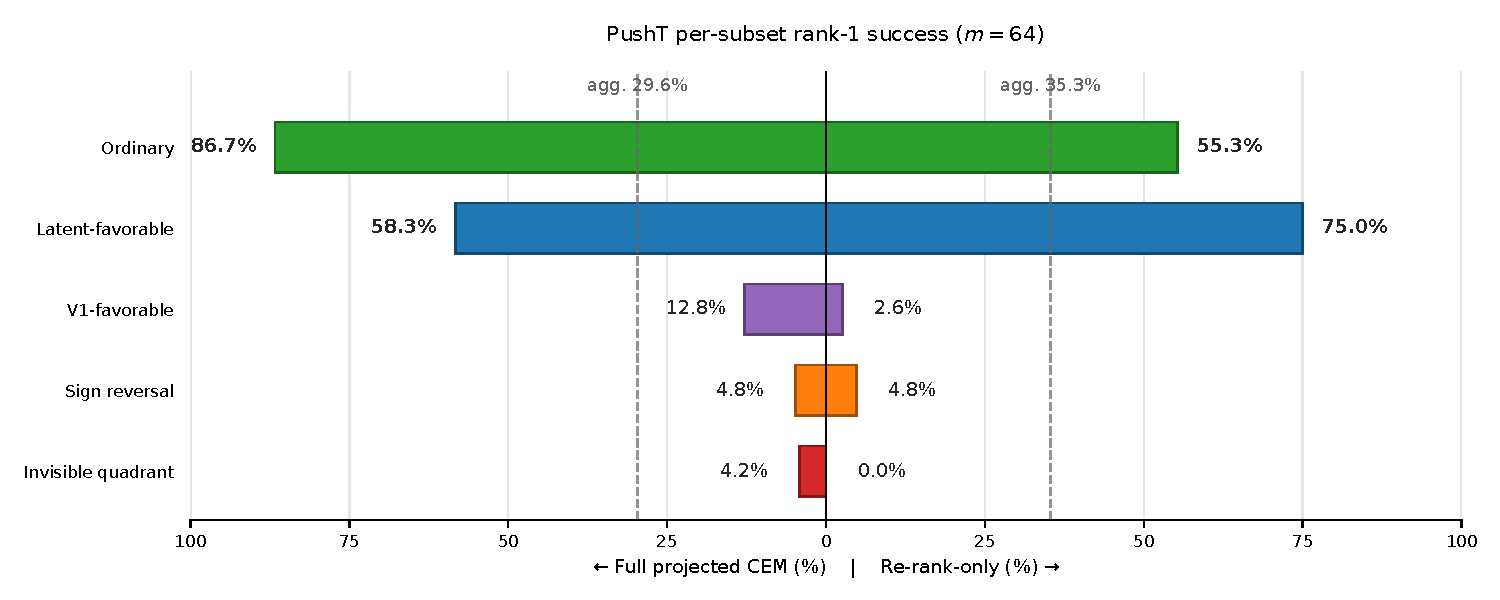
\includegraphics[width=0.9\textwidth]{figures/fig4_butterfly.pdf}
\caption{Per-subset rank-1 planning success at $m = 64$ under two PushT protocols, displayed as a butterfly chart. Left bars show full projected CEM; right bars show re-rank-only. Dashed lines indicate aggregate success. Invisible-quadrant and sign-reversal pairs fail under both protocols, while ordinary and latent-favorable pairs show protocol-dependent differences.}
\label{fig:butterfly_appendix}
\end{figure}

Invisible-quadrant and sign-reversal pairs fail under both protocols.
Ordinary pairs reach 86.7\% under full projected CEM but only 55.3\% under
re-rank-only, suggesting that projected search, not only projected
selection, benefits these pairs.  Latent-favorable pairs show the opposite
pattern: 75.0\% under re-rank-only versus 58.3\% under full projected CEM,
consistent with default CEM producing a better pool for those cases.  This
per-subset decomposition complements the aggregate flatness in
Appendix~\ref{app:stage1b_pusht_rerank} and shows that subset effects
partially cancel in aggregate.

\subsection{Taxonomy Distribution}
\label{app:stage1b_taxonomy}

Across 122 taxonomy cells, the case distribution is A=18, B=8, C=10, E=4,
and unclassified=82.  Case~A, where endpoint geometry transfers to
planning, appears mainly in PushT ordinary and latent-favorable cells at
medium-to-high dimensions.  Case~B, rank-insensitive success, covers Cube
full projected CEM cells; Case~C, endpoint failure as a planning signal,
covers PushT failure subsets.  Case~E, rank-insensitive success in a
locally sufficient pool, is stable: the PushT re-rank-only ordinary subset
passes the tolerant Case~E criterion at $m=64$.  Case~D, emergent local
geometry despite weak endpoint ranking, is not observed.  These categories
instantiate the taxonomy summarized in Table~3.

\section{Negative Result Details}
\label{app:negative}

Section~6 and Figure~5 summarize four failed repairs.  This appendix
provides the corresponding experimental details, full data tables, and
additional ablations.  Unless otherwise noted, all repairs use the same
Track~A 100-pair PushT artifact (Appendix~\ref{app:track_a}) and the
default CEM hyperparameters: 300 samples, 30 elites, and 30 iterations.

\subsection{Learned Cost Heads}
\label{app:negative_cost_heads}

MLP cost heads $C_\psi(z,\zgoal)$ were trained on frozen LeWM latents using
V1 hinge labels.  Two data splits were used: Split~1 contains 15 easier
pairs with at least one successful action under default CEM, and Split~3
contains 16 hard pairs with zero successes under default CEM.  The split
numbering follows internal experiment IDs.

\begin{table}[h]
\centering
\caption{Endpoint ranking on Split~1 held-out pairs.}
\label{tab:h-cost-split1}
\small
\begin{tabular}{lcc}
\toprule
Cost function & Spearman & Pairwise accuracy \\
\midrule
Euclidean & 0.599 & 0.681 \\
Small $C_\psi$ & 0.442 & 0.777 \\
Large $C_\psi$ & 0.512 & 0.812 \\
\bottomrule
\end{tabular}
\end{table}

\begin{table}[h]
\centering
\caption{Predicted endpoint metrics on Split~3 hard pairs across
cost-head variants.}
\label{tab:h-cost-split3}
\small
\begin{tabular}{lcc}
\toprule
Cost function & Spearman & Pairwise accuracy \\
\midrule
Euclidean & 0.233 & 0.578 \\
MLP offline small & 0.270 & 0.614 \\
MLP offline large & 0.352 & 0.611 \\
MLP mixed small & 0.285 & 0.594 \\
MLP mixed temp & 0.378 & 0.597 \\
Mahalanobis low-rank & 0.301 & 0.614 \\
CEM-aware & 0.227 & 0.579 \\
\bottomrule
\end{tabular}
\end{table}

\begin{table}[h]
\centering
\caption{CEM planning success with learned cost heads.  No variant recovers
Split~3 hard-pair successes.}
\label{tab:h-cost-planning}
\small
\begin{tabular}{llcc}
\toprule
Split & Cost & Successes & Total \\
\midrule
Split~3 & Euclidean & 0 & 16 \\
Split~3 & Small $C_\psi$ & 0 & 16 \\
Split~3 & Large $C_\psi$ & 0 & 16 \\
Split~3 & Mixed $C_\psi$ & 0 & 16 \\
Split~3 & Mahalanobis & 0 & 16 \\
Split~3 & CEM-aware & 1 & 16 \\
Split~1 & Euclidean & 4 & 15 \\
Split~1 & $C_\psi$ & 3 & 15 \\
Split~1 & CEM-aware & 2 & 15 \\
\bottomrule
\end{tabular}
\end{table}

The mechanism is elite-cost compression.  At CEM iteration~30, the
Euclidean cost has elite standard deviation 0.354, while $C_\psi$ has elite
standard deviation 0.0015, a 238$\times$ compression.  This removes local
discrimination: all 30 elites receive nearly identical scores, so the
proposal update receives no gradient to separate near-successes from
near-misses, analogous to the V2 indicator degeneracy
(Appendix~\ref{app:oracle}).

\subsection{DINOv2 Encoder Replacement}
\label{app:negative_dinov2}

\begin{table}[h]
\centering
\caption{Endpoint ranking comparison between trained LeWM,
random-projected LeWM, and DINOv2 features on the Track~A 100-pair
artifact.}
\label{tab:h-dino}
\small
\begin{tabular}{lcccc}
\toprule
Representation & Dim & Spearman & Pairwise acc. & Per-pair $\rho$ \\
\midrule
LeWM (trained) & 192 & 0.503 & 0.647 & 0.355 \\
Random projection of LeWM & 192 & 0.501 & 0.643 & 0.349 \\
DINOv2 mean-pool & 768 & 0.261 & 0.610 & 0.285 \\
DINOv2 CLS & 768 & 0.239 & 0.594 & 0.248 \\
\bottomrule
\end{tabular}
\end{table}

DINOv2 mean-pool reaches the highest pairwise accuracy among non-LeWM
representations (0.610), but its Spearman correlation (0.261) is roughly
half of trained LeWM (0.503).  The random projection of LeWM latents
preserves 99.6\% of the Spearman signal (0.501 vs.\ 0.503), consistent
with Stage~1A (Appendix~\ref{app:stage1a}).  The 86.6M-parameter
ViT-B/14 of DINOv2 has 15.7$\times$ more parameters than the 5.5M-parameter
ViT-tiny, so the gap is not attributable to model capacity but to
task-specific training.

\subsection{Hybrid CEM Oracle Budget}
\label{app:negative_hybrid}

Hybrid CEM re-ranks the top $k$ CEM candidates per iteration using the V1
simulator cost from Equation~\ref{eq:v1}.  This tests whether injecting
ground-truth cost signal during search recovers hard-pair successes.

\begin{table}[h]
\centering
\caption{Hybrid CEM successes on Split~3 hard pairs by oracle budget.
Oracle budget is $k/N$ where $N=300$.}
\label{tab:h-oracle-split3}
\small
\begin{tabular}{cccc}
\toprule
$k$ & Oracle budget (\%) & Euclidean pre. & $C_\psi$ pre. \\
\midrule
0 & 0 & 0/16 & 0/16 \\
30 & 10 & 0/16 & 0/16 \\
60 & 20 & 7/16 & 6/16 \\
90 & 30 & 10/16 & 9/16 \\
150 & 50 & 12/16 & 14/16 \\
300 & 100 & 13/16 & 13/16 \\
\bottomrule
\end{tabular}
\end{table}

\begin{table}[h]
\centering
\caption{Partial oracle schedules at $k=60$ on Split~3 hard pairs.  Only
sustained oracle access across all iterations recovers substantial
successes.}
\label{tab:h-oracle-partial}
\small
\begin{tabular}{lc}
\toprule
Schedule & Successes / 16 \\
\midrule
First iteration only & 0 \\
Early 5 iterations & 0 \\
Early 10 iterations & 2 \\
Every 3rd iteration & 4 \\
Late 10 iterations & 3 \\
All 30 iterations & 7 \\
\bottomrule
\end{tabular}
\end{table}

\begin{table}[h]
\centering
\caption{Hybrid CEM successes on Split~1 easier pairs.  Euclidean prefilter
saturates at $k=150$.}
\label{tab:h-oracle-split1}
\small
\begin{tabular}{ccc}
\toprule
$k$ & Euclidean pre. & $C_\psi$ pre. ($k=150$) \\
\midrule
0 & 4/15 & -- \\
60 & 10/15 & -- \\
90 & 12/15 & -- \\
150 & 13/15 & 11/15 \\
300 & 13/15 & -- \\
\bottomrule
\end{tabular}
\end{table}

The 20\% oracle budget threshold ($k=60$) reported in Section~6.3
corresponds to 115{,}200 oracle rollouts and 2{,}880{,}000 simulator
environment steps over 30 CEM iterations.  This overhead makes hybrid CEM
impractical for deployment but confirms that the CEM cost landscape, not
action sampling, is the primary bottleneck.

\subsection{Subspace-CEM Stage A}
\label{app:negative_subspace}

Subspace-CEM searched with an $m=64$ projected cost and selected the rank-1
action by full 192-dimensional LeWM cost.  The locked Stage~A criterion
required at least +3 percentage points over the better of default CEM and
pure projected $m=64$.

\begin{table}[h]
\centering
\caption{Subspace-CEM Stage~A results over 30 pairs and two seeds.  Overall
$\Delta=-8.3$ percentage points versus default CEM.}
\label{tab:h-subspace}
\small
\begin{tabular}{lccc}
\toprule
Subset & Subspace (\%) & Default (\%) & Pure proj. $m{=}64$ (\%) \\
\midrule
Invisible quadrant & 0.0 & 0.0 & 6.25 \\
Ordinary & 75.0 & 83.3 & 85.0 \\
Latent favorable & 90.0 & 100.0 & 80.0 \\
V1 favorable & 20.0 & 40.0 & 20.0 \\
Overall & 48.3 & 56.7 & 50.0 \\
\bottomrule
\end{tabular}
\end{table}

Subspace-CEM regresses in every subset where default CEM has nonzero
success.  The largest regressions are in ordinary pairs ($-8.3$ percentage
points) and V1-favorable pairs ($-20.0$ percentage points).  The failure
shows that projected-cost search moves the CEM pool into a region that
full-dimensional re-ranking cannot recover, confirming that the
search-selection split identified in Section~4 cannot be repaired by a
simple two-stage approach.

\subsection{Cube Anomaly Multi-Seed Check}
\label{app:negative_cube_anomaly}

The Cube full projected CEM dimension sweep (Appendix~\ref{app:stage1b},
Section~G.3) showed a non-monotonic inverted-U success pattern peaking at
$m=32$.  A multi-seed sanity check added projection seeds~1 and~2 to the
existing seed~0 baseline.

\begin{table}[h]
\centering
\caption{Cube full projected CEM multi-seed check over 25 pairs.  The
$m=32$ versus $m=192$ gap is +5.33 percentage points across three seeds.}
\label{tab:h-cube-anomaly}
\small
\begin{tabular}{ccccc}
\toprule
$m$ & Seed 0 (\%) & Seed 1 (\%) & Seed 2 (\%) & 3-seed mean (\%) \\
\midrule
32 & 76.0 & 72.0 & 64.0 & 70.7 \\
192 & 60.0 & 64.0 & 72.0 & 65.3 \\
\bottomrule
\end{tabular}
\end{table}

The $m=32$ advantage over $m=192$ persists across seeds but with high
variance, including a seed-level range of 12 percentage points at $m=32$.
The closeout classified this as MIXED under the pre-registered
5--10 percentage-point criterion.  The final 50-pair, three-seed Cube
extension in Table~\ref{tab:cem-gap-protocols} supersedes the intermediate
$m=64$ sanity row from this check and reports 56.0\% rank-1 success.

\section{Pre-registration Artifacts and Decision Memos}
\label{app:preregistration}

The audit used binding decision trees, fixed evaluation artifacts, and
documented framing resets (Section~3).  Each phase recorded its
hypothesis, continuation criteria, and possible outcomes before data
inspection.  This appendix catalogs the decision memos released with the
supplementary materials and lists the git timestamps that anchor each
pre-registered decision.  Table~\ref{tab:appendix-commits} in
Appendix~\ref{app:reproducibility} provides the commit hashes for the main
experimental artifacts.
Pre-registration follows the broader practice of recording planned hypotheses,
inclusion rules, and analyses before data inspection \citep{hofman2023preregistration}.

\subsection{Audit Trajectory}

Phase 0 reproduced the LeWM PushT baseline and evaluated longer goals:
success fell from 96\% at offset 25 to 58\%, 16\%, and 10\% at offsets 50,
75, and 100.  At offset 50,
$\mathrm{corr}(\Cmodel,C_\mathrm{real\_z})=0.864$, but
encoder-physics alignment varied by pair.

Phase 1 established the Track A artifact: 100 stratified PushT pairs and 80
candidate actions per pair.  The largest-displacement row had the strongest
encoder-physics alignment, with D3 Pearson correlation 0.630, falsifying
large-displacement encoder collapse and moving the audit toward
cost-landscape mismatch.

Phase 2 rejected an architecture-only account when C6 reached Spearman
$-0.200$, while same-dimensional Gaussian projections preserved much of the
trained LeWM ranking signal.  Protocol matching then separated search from
selection: PushT re-rank-only stayed flat from 33.0\% at $m=8$ to 34.0\%
at $m=192$, while full projected CEM rose from 20.6\% to 34.4\%.  The
remaining diagnostic was $\DeltaCEM=\Rendpoint-\Rpool$, the gap between
fixed endpoint geometry and CEM-local pool geometry.

\begin{table*}[h]
\centering
\small
\resizebox{\textwidth}{!}{%
\begin{tabular}{L{0.15\linewidth} L{0.30\linewidth} L{0.31\linewidth} L{0.18\linewidth}}
\toprule
Phase & Hypothesis & Data verdict & Action taken \\
\midrule
Phase 0 & Encoder collapse under large displacement & Case B/E hybrid & Proceed to Track A \\
Phase 1 Track A & Large-displacement encoder is worst & FALSIFIED: D3 best-aligned & Revise to cost-landscape mismatch \\
Cost-head experiment & Learned cost head fixes CEM & FAILED: 0/16 Split 3 & Drop cost-head approach \\
Encoder replacement & DINOv2 encoder fixes ranking & FAILED: 0.286 vs 0.506 & Drop encoder replacement \\
Random-geometry controls & Random architecture-matched geometry explains LeWM endpoint ranking & REJECTED: C6 = -0.200 & Proceed to Plan A evaluation paper \\
Protocol matching & Re-rank flat + CEM has elbow & CONFIRMED: Row 1 & Launch Subspace-CEM smoke \\
Subspace-CEM test & Subspace-CEM beats default by $\geq 3$pp & FAILED: -8.3pp & Drop Subspace-CEM \\
\bottomrule
\end{tabular}}
\caption{Pre-registered decision trace for the audit. Each transition was
determined by a pre-specified gate before the next phase.}
\label{tab:decision-trace}
\end{table*}

\subsection{Decision Memo Index}

\begin{table}[h]
\centering
\small
\setlength{\tabcolsep}{3pt}
\begin{tabular}{@{}p{0.17\textwidth} p{0.32\textwidth} p{0.15\textwidth} p{0.23\textwidth}@{}}
\toprule
Memo & Path & Phase & Verdict \\
\midrule
Stage 1A result memo & \path{docs/phase2/stage1/stage1a_result_memo.md} & Stage 1A & Strong B ruled out; C6 = $-0.200$; proceed to Plan A \\
C6 audit memo & \path{docs/phase2/c6_audit_memo.md} & C6 audit & C6-REAL: anti-correlation confirmed across 10 seeds \\
Cube C6 audit memo & \path{docs/phase2/cube/cube_c6_audit_memo.md} & Cube C6 & C6-NO-INVERSION: Cube randomly initialized encoder is $+0.115 \pm 0.016$ \\
Stage 1B smoke memo & \path{docs/phase2/stage1b_smoke_memo.md} & Stage 1B smoke & Continue B: proceed to full sweep \\
Track B memo & \path{docs/phase2/track_b_memo.md} & Track B & DINOv2 underperforms LeWM ($0.261$ vs.\ $0.503$) \\
P2-0 memo & \path{docs/phase2/p2_0_memo.md} & Learned costs & Cost heads fail planning ($0/16$ Split 3); drop cost-head approach \\
Protocol matching memo & \path{docs/phase2/protocol_matching_memo.md} & Protocol match & Re-rank flat confirmed; Case E stable; launch Subspace-CEM \\
Cube Stage 1B memo & \path{docs/phase2/cube/cube_stage1b_memo.md} & Cube Stage 1B & CUBE-STAGE1B-FLAT-ROBUST \\
Phase A memo & \path{docs/phase2/phase_a_memo.md} & Closeout Phase A & Subspace-CEM FAIL ($-8.3$ pp); Cube anomaly MIXED \\
\bottomrule
\end{tabular}
\caption{Decision memos released with the supplementary materials.  Each
memo was committed before the next experimental phase.}
\label{tab:decision-memo-index}
\end{table}

\subsection{Pre-registered Decision Gates}

\begin{table}[h]
\centering
\footnotesize
\setlength{\tabcolsep}{3pt}
\begin{tabular}{@{}p{0.17\textwidth} p{0.33\textwidth} p{0.27\textwidth} p{0.11\textwidth}@{}}
\toprule
Gate & Pre-registered criterion & Observed value & Outcome \\
\midrule
Strong B (Stage 1A) & $m \leq 8$ projection within $0.05$ Spearman of C0 and C6 within $0.05$ of C0 & C2 $m{=}8$ gap $= 0.127$; C6 $= -0.200$ & Ruled out \\
Learned cost planning (P2-0) & $\geq 5/16$ Split 3 hard-pair rescues without regression & Best variant: $1/16$ (CEM-aware) & Failed \\
DINOv2 encoder (Track B) & DINOv2 matches LeWM Spearman within $0.05$ & Gap $= 0.242$ ($0.261$ vs.\ $0.503$) & Failed \\
Protocol matching & Re-rank-only flat ($< 5$ pp range) and full projected CEM has elbow & Re-rank range $= 5.4$ pp; CEM elbow confirmed & Confirmed \\
Subspace-CEM Stage A & $\geq +3$ pp over the better of default and pure projected $m{=}64$ & $-8.3$ pp vs.\ default & Failed \\
Cube anomaly & $m{=}32$ vs.\ $m{=}192$ gap $\geq 10$ pp across 3 seeds & $+5.33$ pp (MIXED: in 5--10 pp range) & Mixed \\
\bottomrule
\end{tabular}
\caption{Pre-registered decision gates with quantitative thresholds.  Each
gate was recorded in the corresponding memo before data inspection.}
\label{tab:preregistered-gates}
\end{table}

\subsection{Git-Anchored Timeline}

\begin{table}[h]
\centering
\footnotesize
\setlength{\tabcolsep}{4pt}
\begin{tabular}{@{}p{0.22\textwidth} p{0.13\textwidth} p{0.55\textwidth}@{}}
\toprule
Date & Commit & Event \\
\midrule
2026-05-01 03:36 & \texttt{486adee} & Aggregate latent diagnostics and Cube eval pipeline \\
2026-05-01 03:52 & \texttt{eac7bfc} & Cube baseline and sweep infrastructure \\
2026-05-01 13:06 & \texttt{7388a9a} & Phase 0 three-cost refactor \\
2026-05-01 18:03 & \texttt{78900c3} & Track A D3-row cost-criterion ablation (V1/V2/V3) \\
2026-05-01 22:53 & \texttt{ecea011} & Track A closeout \\
2026-05-02 17:08 & \texttt{e1f97f3} & Stage 1A random-geometry decision gate \\
2026-05-02 19:25 & \texttt{dac7a06} & C6 audit S1--S6 + memo (verdict: C6-REAL) \\
2026-05-02 20:58 & \texttt{e2e19e3} & Stage 1B smoke memo (verdict: Continue B) \\
2026-05-03 14:29 & \texttt{2fdee8e} & Taxonomy, hero figure, protocol memo \\
2026-05-03 & \texttt{adc573ac} & Subspace-CEM Stage A (verdict: FAIL) \\
\bottomrule
\end{tabular}
\caption{Git-anchored audit timeline.  Commits are listed in chronological
order; each records the pre-registered decision or artifact before the
subsequent phase.}
\label{tab:git-anchored-timeline}
\end{table}

\subsection{Framing Resets}

The audit underwent three documented framing resets.  The
first reset moved from encoder-collapse to cost-landscape mismatch after
Phase 1 falsified the large-displacement hypothesis.  The second narrowed
cost-landscape mismatch to endpoint-planning decoupling after C6 rejected
the architecture-only account.  The third incorporated the search-selection
split after protocol matching confirmed the re-rank flatness.  Each reset
was written into a memo before the next phase's experiments.


\end{document}
